\documentclass[11pt]{amsart}
\usepackage[margin=1in]{geometry}
\usepackage{amsmath,amssymb,amsthm,mathtools}
\usepackage{enumitem}
\usepackage{tikz}
\usetikzlibrary{positioning,arrows.meta,calc,fit,shapes.geometric}
\usepackage{hyperref}
\hypersetup{colorlinks=true,linkcolor=blue,citecolor=blue,urlcolor=blue}
\usepackage[final]{microtype}
\setlength{\emergencystretch}{3em}
\usepackage{setspace}
\setstretch{1.14}
\newcommand{\leanrepo}{https://github.com/HQIV/hqiv-lean/blob/main}
% Lean module / identifier helpers: visible text is rendered with \nolinkurl
% so that slashes, underscores, and dots become legal break points.
\newcommand{\leanfile}[1]{\href{\leanrepo/#1}{\nolinkurl{#1}}}
\newcommand{\leanid}[1]{\nolinkurl{#1}}

\title[Octonionic Action and Uniqueness]{Octonionic Action from the HQIV-LEAN Variational Layer:\\
Derivation, Holonomy Alignment, and a Tiered Uniqueness Thesis}
\author{Steven Ettinger Jr}
\address{Independent Researcher}
\email{steven@disregardfiat.tech}
\date{Published v1 --- Zenodo \href{https://doi.org/10.5281/zenodo.20416085}{10.5281/zenodo.20416085} (2026-05-27); manuscript Preprint v3}

\newtheorem{theorem}{Theorem}[section]
\newtheorem{lemma}[theorem]{Lemma}
\newtheorem{proposition}[theorem]{Proposition}
\newtheorem{corollary}[theorem]{Corollary}
\newtheorem{definition}[theorem]{Definition}
\newtheorem{remark}[theorem]{Remark}
\newtheorem{conjecture}[theorem]{Conjecture}
\newtheorem{example}[theorem]{Example}

\begin{document}

\begin{abstract}
This manuscript is a variational sequel to \cite{hqiv-so8-paper} and \cite{hqiv-3d-growth-paper}. Those works package discrete null-shell growth, a normalized cumulative phase readout \(\mathcal{R}\), an explicit phase-lift generator \(\Delta\), and machine-checked Lie closure \(G_2\cup\{\Delta\}\Rightarrow\mathfrak{so}(8)\) on the HQVM octonionic seed. Here we centre the \emph{action} layer already present in the HQIV-LEAN library: a discrete octonion-indexed gauge potential \(A^a{}_\mu\), field strength \(F^a{}_{\mu\nu}\), an O--Maxwell Lagrangian, an Euler--Lagrange covector that matches the discrete divergence of \(F\) minus sources, a gravitational constraint action tied to the HQVM Friedmann identity, and the holonomy glue that re-packages the \emph{same} \(F\) data as abelian plaquette transports with a proved cyclic Stokes identity. The holonomy bridge ties the variational kinetic aggregate to Wilson-type defects on the minimal \(\mathrm{Fin}\,4\) cycle without changing the underlying discrete flux---the same bookkeeping the rapidity layer uses before Lie closure.

The proved core is precise about its honesty boundary: the Euler--Lagrange identity, the cyclic flux sum, two-sided bounds comparing the kinetic aggregate to cyclic Wilson squares, and the equivalence of the gravitational constraint with the HQVM Friedmann identity all live as zero-\texttt{sorry} Lean theorems in the public slimmed mirror \cite{hqiv-lean}; literature-translation maps (calculation-approximation rewrites of discrete objects in standard notation), patch-extension wrappers, and discrete-measure choices remain narrative or scaffolded and are explicitly labelled as such throughout. The \emph{tiered uniqueness thesis} is the paper's conceptual payoff: \textbf{(I)}~within the declared polynomial gauge ansatz, the discrete EL slot is the exact finite-difference analogue of the continuum Maxwell pattern; \textbf{(II)}~Hurwitz rigidity and eight-dimensional division-algebra uniqueness align the \(\mathrm{Fin}\,8\) carrier with triality/\(\mathrm{Spin}(8)\) and the certified \(G_2\cup\{\Delta\}\) seed; \textbf{(III)}~a structured patch-interoperability programme (calculation-approximation translations, paired patch stationarity for the gauge/gravity sectors, associator-weighted discrete measure) replaces a single vague conjecture. Following the patch-theory reader contract, the observable universe \emph{is} the whole universe in the HQIV ontology, so no continuum limit is required---and in several load-bearing places, taking one would erase the discrete index that does the predictive work; continuum formulas are at most calculation-approximation coordinates used for cross-citation, not refinements. For readers from lattice gauge theory, the holonomy lemmas position the same \(F\) slots where Wilson plaquette language applies \cite{wilson1974,creutz1983}. We also name \emph{lapse dragging}: the HQVM identification of the cumulative lapse increment \(\phi t/c\) above the Newtonian \(\Phi\) piece with the \emph{same} auxiliary scalar that enters the action's \(\phi\)-coupling and the effective gravitational coupling \(G_{\mathrm{eff}}(\phi)=\phi^{3/5}\); Remark~\ref{rem:lapse-lambda} records sample \(G_{\mathrm{eff}}/G_0\) ratios and links that single-\(\alpha\) pipeline to galactic rotation-curve phenomenology, with a quantitative SPARC-style first pass in Table~\ref{tab:sparc-firstpass} (Jacobson/Brodie horizon picture \cite{jacobson1995,brodie2026,lelli2016sparc}). All Lean module paths and identifiers are collected in Appendix~\ref{app:lean-index}; the body uses reader-friendly names that hyperlink there.
\end{abstract}
\maketitle

% Shared reader contract: patch QFT + discrete numerics.
% From papers/*.tex:     % Shared reader contract: patch QFT + discrete numerics.
% From papers/*.tex:     % Shared reader contract: patch QFT + discrete numerics.
% From papers/*.tex:     \input{include/patch_theory_messaging.tex}
% From papers/paper/*.tex: \input{../include/patch_theory_messaging.tex}

\paragraph{Patch QFT and discrete numerics (reader contract).}
HQIV (Horizon-Quantized Informational Vacuum) is formulated as a \emph{patch theory}: quantum fields, actions, and physical readouts are attached to discrete patches---shell indices $m\in\mathbb{N}$, finite spacetime index types (e.g.\ $\mathrm{Fin}\,4$), and horizon-limited charts---rather than to a hypothetical fundamental smooth spacetime obtained as a mesh-refinement or ultraviolet limit.
Accordingly, when this text refers to ``QFT,'' it means \emph{patch QFT}: patching rules, finite measurement ledgers, and variational identities on the discrete spine; it is not the claim that the theory is \emph{defined} by recovering ordinary continuum quantum field theory through such a limit.
The numbers that admit the sharpest statements---mass and coupling ladders, curvature ratios, shell thermodynamics, and rational witnesses in \texttt{HQIV\_LEAN}---are objects of \emph{discrete mathematics} on $\mathbb{N}$ (combinatorial growth, cumulative simplex ledgers) together with the ordered field $\mathbb{R}$ as used in the proof assistant for analysis, bounds, and phenomenological display.
Smooth-manifold or continuum field notation, when it appears, is a \emph{translation layer} for comparison with standard physics literature; it does not supersede the discrete definitions.

\paragraph{A continuum is not required, and in places would destroy these results.}
The discrete patch layer is \emph{not} a numerical approximation to a more fundamental continuum theory awaiting future construction; it is the ontology.  Where the literature treats ``the continuum limit'' as the goal, HQIV treats it as a \emph{calculation approximation} for comparison with standard formulas.  The continuum form is an optional convenience for comparison; the proved discrete statement is what carries the physics.  In several load-bearing places---the curvature imprint $\delta_E(m)$ at shell $m$, the harmonic ladder masses $m_\tau\to m_\mu\to m_e$, the lock-in vev $v=\sqrt{\eta_{\rm paper}\,\Omega_k(m_{\rm lockin};m_{\rm lockin})}$, the proton anchor at $m=\mathrm{referenceM}=4$, the baryon-asymmetry $\eta\propto 6^7\sqrt{3}/(m+1)$, and the rational coefficients $\alpha=3/5$, $\gamma=2/5$, $\alpha_{\rm GUT}=1/42$---taking a literal $m\to\infty$ or sub-Planck continuum limit would \emph{erase} the discrete index that is doing the predictive work.  Continuum forms of these objects are therefore not preferred refinements; they are degenerate, information-losing readouts of the same patch data.

\paragraph{An exception: $\mathfrak{so}(8)$ as a de-facto continuum algebra from a discrete construction.}
Principled exception to the discrete-only stance: the closed Lie algebra $\mathfrak{so}(8) \supseteq G_2\cup\{\Delta\}$ generated from the Fano octonion left-multiplication table and the phase-lift generator $\Delta\in(\mathrm{e}_1,\mathrm{e}_7)$.  Although $\mathfrak{so}(8)$ is a continuous (28-dimensional real) Lie algebra, it is built here entirely from \emph{discrete} ingredients (the seven imaginary octonion units, a finite Fano table, and one $\pi/2$ rotation), and its closure to 28 dimensions is a finite linear-algebra certificate (see the \texttt{Hqiv.SO8Closure} / \texttt{Hqiv.SO8ClosureInterface} stack).  The Lie-group structure is therefore a \emph{de-facto continuum algebra obtained from a discrete construction}: continuous in parameter space, but with no continuum spacetime, no continuum measure, and no UV limit attached.  When this manuscript or its companions write $\exp(t\,\Delta)\in\mathrm{SO}(8)$ or treat $\mathfrak{so}(8)$ rotations as smooth, those are statements internal to a finite-dimensional Lie group whose generators are certified by discrete data; they are \emph{not} a continuum-spacetime commitment and do not require a continuum-QFT scaffolding.

% From papers/paper/*.tex: % Shared reader contract: patch QFT + discrete numerics.
% From papers/*.tex:     \input{include/patch_theory_messaging.tex}
% From papers/paper/*.tex: \input{../include/patch_theory_messaging.tex}

\paragraph{Patch QFT and discrete numerics (reader contract).}
HQIV (Horizon-Quantized Informational Vacuum) is formulated as a \emph{patch theory}: quantum fields, actions, and physical readouts are attached to discrete patches---shell indices $m\in\mathbb{N}$, finite spacetime index types (e.g.\ $\mathrm{Fin}\,4$), and horizon-limited charts---rather than to a hypothetical fundamental smooth spacetime obtained as a mesh-refinement or ultraviolet limit.
Accordingly, when this text refers to ``QFT,'' it means \emph{patch QFT}: patching rules, finite measurement ledgers, and variational identities on the discrete spine; it is not the claim that the theory is \emph{defined} by recovering ordinary continuum quantum field theory through such a limit.
The numbers that admit the sharpest statements---mass and coupling ladders, curvature ratios, shell thermodynamics, and rational witnesses in \texttt{HQIV\_LEAN}---are objects of \emph{discrete mathematics} on $\mathbb{N}$ (combinatorial growth, cumulative simplex ledgers) together with the ordered field $\mathbb{R}$ as used in the proof assistant for analysis, bounds, and phenomenological display.
Smooth-manifold or continuum field notation, when it appears, is a \emph{translation layer} for comparison with standard physics literature; it does not supersede the discrete definitions.

\paragraph{A continuum is not required, and in places would destroy these results.}
The discrete patch layer is \emph{not} a numerical approximation to a more fundamental continuum theory awaiting future construction; it is the ontology.  Where the literature treats ``the continuum limit'' as the goal, HQIV treats it as a \emph{calculation approximation} for comparison with standard formulas.  The continuum form is an optional convenience for comparison; the proved discrete statement is what carries the physics.  In several load-bearing places---the curvature imprint $\delta_E(m)$ at shell $m$, the harmonic ladder masses $m_\tau\to m_\mu\to m_e$, the lock-in vev $v=\sqrt{\eta_{\rm paper}\,\Omega_k(m_{\rm lockin};m_{\rm lockin})}$, the proton anchor at $m=\mathrm{referenceM}=4$, the baryon-asymmetry $\eta\propto 6^7\sqrt{3}/(m+1)$, and the rational coefficients $\alpha=3/5$, $\gamma=2/5$, $\alpha_{\rm GUT}=1/42$---taking a literal $m\to\infty$ or sub-Planck continuum limit would \emph{erase} the discrete index that is doing the predictive work.  Continuum forms of these objects are therefore not preferred refinements; they are degenerate, information-losing readouts of the same patch data.

\paragraph{An exception: $\mathfrak{so}(8)$ as a de-facto continuum algebra from a discrete construction.}
Principled exception to the discrete-only stance: the closed Lie algebra $\mathfrak{so}(8) \supseteq G_2\cup\{\Delta\}$ generated from the Fano octonion left-multiplication table and the phase-lift generator $\Delta\in(\mathrm{e}_1,\mathrm{e}_7)$.  Although $\mathfrak{so}(8)$ is a continuous (28-dimensional real) Lie algebra, it is built here entirely from \emph{discrete} ingredients (the seven imaginary octonion units, a finite Fano table, and one $\pi/2$ rotation), and its closure to 28 dimensions is a finite linear-algebra certificate (see the \texttt{Hqiv.SO8Closure} / \texttt{Hqiv.SO8ClosureInterface} stack).  The Lie-group structure is therefore a \emph{de-facto continuum algebra obtained from a discrete construction}: continuous in parameter space, but with no continuum spacetime, no continuum measure, and no UV limit attached.  When this manuscript or its companions write $\exp(t\,\Delta)\in\mathrm{SO}(8)$ or treat $\mathfrak{so}(8)$ rotations as smooth, those are statements internal to a finite-dimensional Lie group whose generators are certified by discrete data; they are \emph{not} a continuum-spacetime commitment and do not require a continuum-QFT scaffolding.


\paragraph{Patch QFT and discrete numerics (reader contract).}
HQIV (Horizon-Quantized Informational Vacuum) is formulated as a \emph{patch theory}: quantum fields, actions, and physical readouts are attached to discrete patches---shell indices $m\in\mathbb{N}$, finite spacetime index types (e.g.\ $\mathrm{Fin}\,4$), and horizon-limited charts---rather than to a hypothetical fundamental smooth spacetime obtained as a mesh-refinement or ultraviolet limit.
Accordingly, when this text refers to ``QFT,'' it means \emph{patch QFT}: patching rules, finite measurement ledgers, and variational identities on the discrete spine; it is not the claim that the theory is \emph{defined} by recovering ordinary continuum quantum field theory through such a limit.
The numbers that admit the sharpest statements---mass and coupling ladders, curvature ratios, shell thermodynamics, and rational witnesses in \texttt{HQIV\_LEAN}---are objects of \emph{discrete mathematics} on $\mathbb{N}$ (combinatorial growth, cumulative simplex ledgers) together with the ordered field $\mathbb{R}$ as used in the proof assistant for analysis, bounds, and phenomenological display.
Smooth-manifold or continuum field notation, when it appears, is a \emph{translation layer} for comparison with standard physics literature; it does not supersede the discrete definitions.

\paragraph{A continuum is not required, and in places would destroy these results.}
The discrete patch layer is \emph{not} a numerical approximation to a more fundamental continuum theory awaiting future construction; it is the ontology.  Where the literature treats ``the continuum limit'' as the goal, HQIV treats it as a \emph{calculation approximation} for comparison with standard formulas.  The continuum form is an optional convenience for comparison; the proved discrete statement is what carries the physics.  In several load-bearing places---the curvature imprint $\delta_E(m)$ at shell $m$, the harmonic ladder masses $m_\tau\to m_\mu\to m_e$, the lock-in vev $v=\sqrt{\eta_{\rm paper}\,\Omega_k(m_{\rm lockin};m_{\rm lockin})}$, the proton anchor at $m=\mathrm{referenceM}=4$, the baryon-asymmetry $\eta\propto 6^7\sqrt{3}/(m+1)$, and the rational coefficients $\alpha=3/5$, $\gamma=2/5$, $\alpha_{\rm GUT}=1/42$---taking a literal $m\to\infty$ or sub-Planck continuum limit would \emph{erase} the discrete index that is doing the predictive work.  Continuum forms of these objects are therefore not preferred refinements; they are degenerate, information-losing readouts of the same patch data.

\paragraph{An exception: $\mathfrak{so}(8)$ as a de-facto continuum algebra from a discrete construction.}
Principled exception to the discrete-only stance: the closed Lie algebra $\mathfrak{so}(8) \supseteq G_2\cup\{\Delta\}$ generated from the Fano octonion left-multiplication table and the phase-lift generator $\Delta\in(\mathrm{e}_1,\mathrm{e}_7)$.  Although $\mathfrak{so}(8)$ is a continuous (28-dimensional real) Lie algebra, it is built here entirely from \emph{discrete} ingredients (the seven imaginary octonion units, a finite Fano table, and one $\pi/2$ rotation), and its closure to 28 dimensions is a finite linear-algebra certificate (see the \texttt{Hqiv.SO8Closure} / \texttt{Hqiv.SO8ClosureInterface} stack).  The Lie-group structure is therefore a \emph{de-facto continuum algebra obtained from a discrete construction}: continuous in parameter space, but with no continuum spacetime, no continuum measure, and no UV limit attached.  When this manuscript or its companions write $\exp(t\,\Delta)\in\mathrm{SO}(8)$ or treat $\mathfrak{so}(8)$ rotations as smooth, those are statements internal to a finite-dimensional Lie group whose generators are certified by discrete data; they are \emph{not} a continuum-spacetime commitment and do not require a continuum-QFT scaffolding.

% From papers/paper/*.tex: % Shared reader contract: patch QFT + discrete numerics.
% From papers/*.tex:     % Shared reader contract: patch QFT + discrete numerics.
% From papers/*.tex:     \input{include/patch_theory_messaging.tex}
% From papers/paper/*.tex: \input{../include/patch_theory_messaging.tex}

\paragraph{Patch QFT and discrete numerics (reader contract).}
HQIV (Horizon-Quantized Informational Vacuum) is formulated as a \emph{patch theory}: quantum fields, actions, and physical readouts are attached to discrete patches---shell indices $m\in\mathbb{N}$, finite spacetime index types (e.g.\ $\mathrm{Fin}\,4$), and horizon-limited charts---rather than to a hypothetical fundamental smooth spacetime obtained as a mesh-refinement or ultraviolet limit.
Accordingly, when this text refers to ``QFT,'' it means \emph{patch QFT}: patching rules, finite measurement ledgers, and variational identities on the discrete spine; it is not the claim that the theory is \emph{defined} by recovering ordinary continuum quantum field theory through such a limit.
The numbers that admit the sharpest statements---mass and coupling ladders, curvature ratios, shell thermodynamics, and rational witnesses in \texttt{HQIV\_LEAN}---are objects of \emph{discrete mathematics} on $\mathbb{N}$ (combinatorial growth, cumulative simplex ledgers) together with the ordered field $\mathbb{R}$ as used in the proof assistant for analysis, bounds, and phenomenological display.
Smooth-manifold or continuum field notation, when it appears, is a \emph{translation layer} for comparison with standard physics literature; it does not supersede the discrete definitions.

\paragraph{A continuum is not required, and in places would destroy these results.}
The discrete patch layer is \emph{not} a numerical approximation to a more fundamental continuum theory awaiting future construction; it is the ontology.  Where the literature treats ``the continuum limit'' as the goal, HQIV treats it as a \emph{calculation approximation} for comparison with standard formulas.  The continuum form is an optional convenience for comparison; the proved discrete statement is what carries the physics.  In several load-bearing places---the curvature imprint $\delta_E(m)$ at shell $m$, the harmonic ladder masses $m_\tau\to m_\mu\to m_e$, the lock-in vev $v=\sqrt{\eta_{\rm paper}\,\Omega_k(m_{\rm lockin};m_{\rm lockin})}$, the proton anchor at $m=\mathrm{referenceM}=4$, the baryon-asymmetry $\eta\propto 6^7\sqrt{3}/(m+1)$, and the rational coefficients $\alpha=3/5$, $\gamma=2/5$, $\alpha_{\rm GUT}=1/42$---taking a literal $m\to\infty$ or sub-Planck continuum limit would \emph{erase} the discrete index that is doing the predictive work.  Continuum forms of these objects are therefore not preferred refinements; they are degenerate, information-losing readouts of the same patch data.

\paragraph{An exception: $\mathfrak{so}(8)$ as a de-facto continuum algebra from a discrete construction.}
Principled exception to the discrete-only stance: the closed Lie algebra $\mathfrak{so}(8) \supseteq G_2\cup\{\Delta\}$ generated from the Fano octonion left-multiplication table and the phase-lift generator $\Delta\in(\mathrm{e}_1,\mathrm{e}_7)$.  Although $\mathfrak{so}(8)$ is a continuous (28-dimensional real) Lie algebra, it is built here entirely from \emph{discrete} ingredients (the seven imaginary octonion units, a finite Fano table, and one $\pi/2$ rotation), and its closure to 28 dimensions is a finite linear-algebra certificate (see the \texttt{Hqiv.SO8Closure} / \texttt{Hqiv.SO8ClosureInterface} stack).  The Lie-group structure is therefore a \emph{de-facto continuum algebra obtained from a discrete construction}: continuous in parameter space, but with no continuum spacetime, no continuum measure, and no UV limit attached.  When this manuscript or its companions write $\exp(t\,\Delta)\in\mathrm{SO}(8)$ or treat $\mathfrak{so}(8)$ rotations as smooth, those are statements internal to a finite-dimensional Lie group whose generators are certified by discrete data; they are \emph{not} a continuum-spacetime commitment and do not require a continuum-QFT scaffolding.

% From papers/paper/*.tex: % Shared reader contract: patch QFT + discrete numerics.
% From papers/*.tex:     \input{include/patch_theory_messaging.tex}
% From papers/paper/*.tex: \input{../include/patch_theory_messaging.tex}

\paragraph{Patch QFT and discrete numerics (reader contract).}
HQIV (Horizon-Quantized Informational Vacuum) is formulated as a \emph{patch theory}: quantum fields, actions, and physical readouts are attached to discrete patches---shell indices $m\in\mathbb{N}$, finite spacetime index types (e.g.\ $\mathrm{Fin}\,4$), and horizon-limited charts---rather than to a hypothetical fundamental smooth spacetime obtained as a mesh-refinement or ultraviolet limit.
Accordingly, when this text refers to ``QFT,'' it means \emph{patch QFT}: patching rules, finite measurement ledgers, and variational identities on the discrete spine; it is not the claim that the theory is \emph{defined} by recovering ordinary continuum quantum field theory through such a limit.
The numbers that admit the sharpest statements---mass and coupling ladders, curvature ratios, shell thermodynamics, and rational witnesses in \texttt{HQIV\_LEAN}---are objects of \emph{discrete mathematics} on $\mathbb{N}$ (combinatorial growth, cumulative simplex ledgers) together with the ordered field $\mathbb{R}$ as used in the proof assistant for analysis, bounds, and phenomenological display.
Smooth-manifold or continuum field notation, when it appears, is a \emph{translation layer} for comparison with standard physics literature; it does not supersede the discrete definitions.

\paragraph{A continuum is not required, and in places would destroy these results.}
The discrete patch layer is \emph{not} a numerical approximation to a more fundamental continuum theory awaiting future construction; it is the ontology.  Where the literature treats ``the continuum limit'' as the goal, HQIV treats it as a \emph{calculation approximation} for comparison with standard formulas.  The continuum form is an optional convenience for comparison; the proved discrete statement is what carries the physics.  In several load-bearing places---the curvature imprint $\delta_E(m)$ at shell $m$, the harmonic ladder masses $m_\tau\to m_\mu\to m_e$, the lock-in vev $v=\sqrt{\eta_{\rm paper}\,\Omega_k(m_{\rm lockin};m_{\rm lockin})}$, the proton anchor at $m=\mathrm{referenceM}=4$, the baryon-asymmetry $\eta\propto 6^7\sqrt{3}/(m+1)$, and the rational coefficients $\alpha=3/5$, $\gamma=2/5$, $\alpha_{\rm GUT}=1/42$---taking a literal $m\to\infty$ or sub-Planck continuum limit would \emph{erase} the discrete index that is doing the predictive work.  Continuum forms of these objects are therefore not preferred refinements; they are degenerate, information-losing readouts of the same patch data.

\paragraph{An exception: $\mathfrak{so}(8)$ as a de-facto continuum algebra from a discrete construction.}
Principled exception to the discrete-only stance: the closed Lie algebra $\mathfrak{so}(8) \supseteq G_2\cup\{\Delta\}$ generated from the Fano octonion left-multiplication table and the phase-lift generator $\Delta\in(\mathrm{e}_1,\mathrm{e}_7)$.  Although $\mathfrak{so}(8)$ is a continuous (28-dimensional real) Lie algebra, it is built here entirely from \emph{discrete} ingredients (the seven imaginary octonion units, a finite Fano table, and one $\pi/2$ rotation), and its closure to 28 dimensions is a finite linear-algebra certificate (see the \texttt{Hqiv.SO8Closure} / \texttt{Hqiv.SO8ClosureInterface} stack).  The Lie-group structure is therefore a \emph{de-facto continuum algebra obtained from a discrete construction}: continuous in parameter space, but with no continuum spacetime, no continuum measure, and no UV limit attached.  When this manuscript or its companions write $\exp(t\,\Delta)\in\mathrm{SO}(8)$ or treat $\mathfrak{so}(8)$ rotations as smooth, those are statements internal to a finite-dimensional Lie group whose generators are certified by discrete data; they are \emph{not} a continuum-spacetime commitment and do not require a continuum-QFT scaffolding.


\paragraph{Patch QFT and discrete numerics (reader contract).}
HQIV (Horizon-Quantized Informational Vacuum) is formulated as a \emph{patch theory}: quantum fields, actions, and physical readouts are attached to discrete patches---shell indices $m\in\mathbb{N}$, finite spacetime index types (e.g.\ $\mathrm{Fin}\,4$), and horizon-limited charts---rather than to a hypothetical fundamental smooth spacetime obtained as a mesh-refinement or ultraviolet limit.
Accordingly, when this text refers to ``QFT,'' it means \emph{patch QFT}: patching rules, finite measurement ledgers, and variational identities on the discrete spine; it is not the claim that the theory is \emph{defined} by recovering ordinary continuum quantum field theory through such a limit.
The numbers that admit the sharpest statements---mass and coupling ladders, curvature ratios, shell thermodynamics, and rational witnesses in \texttt{HQIV\_LEAN}---are objects of \emph{discrete mathematics} on $\mathbb{N}$ (combinatorial growth, cumulative simplex ledgers) together with the ordered field $\mathbb{R}$ as used in the proof assistant for analysis, bounds, and phenomenological display.
Smooth-manifold or continuum field notation, when it appears, is a \emph{translation layer} for comparison with standard physics literature; it does not supersede the discrete definitions.

\paragraph{A continuum is not required, and in places would destroy these results.}
The discrete patch layer is \emph{not} a numerical approximation to a more fundamental continuum theory awaiting future construction; it is the ontology.  Where the literature treats ``the continuum limit'' as the goal, HQIV treats it as a \emph{calculation approximation} for comparison with standard formulas.  The continuum form is an optional convenience for comparison; the proved discrete statement is what carries the physics.  In several load-bearing places---the curvature imprint $\delta_E(m)$ at shell $m$, the harmonic ladder masses $m_\tau\to m_\mu\to m_e$, the lock-in vev $v=\sqrt{\eta_{\rm paper}\,\Omega_k(m_{\rm lockin};m_{\rm lockin})}$, the proton anchor at $m=\mathrm{referenceM}=4$, the baryon-asymmetry $\eta\propto 6^7\sqrt{3}/(m+1)$, and the rational coefficients $\alpha=3/5$, $\gamma=2/5$, $\alpha_{\rm GUT}=1/42$---taking a literal $m\to\infty$ or sub-Planck continuum limit would \emph{erase} the discrete index that is doing the predictive work.  Continuum forms of these objects are therefore not preferred refinements; they are degenerate, information-losing readouts of the same patch data.

\paragraph{An exception: $\mathfrak{so}(8)$ as a de-facto continuum algebra from a discrete construction.}
Principled exception to the discrete-only stance: the closed Lie algebra $\mathfrak{so}(8) \supseteq G_2\cup\{\Delta\}$ generated from the Fano octonion left-multiplication table and the phase-lift generator $\Delta\in(\mathrm{e}_1,\mathrm{e}_7)$.  Although $\mathfrak{so}(8)$ is a continuous (28-dimensional real) Lie algebra, it is built here entirely from \emph{discrete} ingredients (the seven imaginary octonion units, a finite Fano table, and one $\pi/2$ rotation), and its closure to 28 dimensions is a finite linear-algebra certificate (see the \texttt{Hqiv.SO8Closure} / \texttt{Hqiv.SO8ClosureInterface} stack).  The Lie-group structure is therefore a \emph{de-facto continuum algebra obtained from a discrete construction}: continuous in parameter space, but with no continuum spacetime, no continuum measure, and no UV limit attached.  When this manuscript or its companions write $\exp(t\,\Delta)\in\mathrm{SO}(8)$ or treat $\mathfrak{so}(8)$ rotations as smooth, those are statements internal to a finite-dimensional Lie group whose generators are certified by discrete data; they are \emph{not} a continuum-spacetime commitment and do not require a continuum-QFT scaffolding.


\paragraph{Patch QFT and discrete numerics (reader contract).}
HQIV (Horizon-Quantized Informational Vacuum) is formulated as a \emph{patch theory}: quantum fields, actions, and physical readouts are attached to discrete patches---shell indices $m\in\mathbb{N}$, finite spacetime index types (e.g.\ $\mathrm{Fin}\,4$), and horizon-limited charts---rather than to a hypothetical fundamental smooth spacetime obtained as a mesh-refinement or ultraviolet limit.
Accordingly, when this text refers to ``QFT,'' it means \emph{patch QFT}: patching rules, finite measurement ledgers, and variational identities on the discrete spine; it is not the claim that the theory is \emph{defined} by recovering ordinary continuum quantum field theory through such a limit.
The numbers that admit the sharpest statements---mass and coupling ladders, curvature ratios, shell thermodynamics, and rational witnesses in \texttt{HQIV\_LEAN}---are objects of \emph{discrete mathematics} on $\mathbb{N}$ (combinatorial growth, cumulative simplex ledgers) together with the ordered field $\mathbb{R}$ as used in the proof assistant for analysis, bounds, and phenomenological display.
Smooth-manifold or continuum field notation, when it appears, is a \emph{translation layer} for comparison with standard physics literature; it does not supersede the discrete definitions.

\paragraph{A continuum is not required, and in places would destroy these results.}
The discrete patch layer is \emph{not} a numerical approximation to a more fundamental continuum theory awaiting future construction; it is the ontology.  Where the literature treats ``the continuum limit'' as the goal, HQIV treats it as a \emph{calculation approximation} for comparison with standard formulas.  The continuum form is an optional convenience for comparison; the proved discrete statement is what carries the physics.  In several load-bearing places---the curvature imprint $\delta_E(m)$ at shell $m$, the harmonic ladder masses $m_\tau\to m_\mu\to m_e$, the lock-in vev $v=\sqrt{\eta_{\rm paper}\,\Omega_k(m_{\rm lockin};m_{\rm lockin})}$, the proton anchor at $m=\mathrm{referenceM}=4$, the baryon-asymmetry $\eta\propto 6^7\sqrt{3}/(m+1)$, and the rational coefficients $\alpha=3/5$, $\gamma=2/5$, $\alpha_{\rm GUT}=1/42$---taking a literal $m\to\infty$ or sub-Planck continuum limit would \emph{erase} the discrete index that is doing the predictive work.  Continuum forms of these objects are therefore not preferred refinements; they are degenerate, information-losing readouts of the same patch data.

\paragraph{An exception: $\mathfrak{so}(8)$ as a de-facto continuum algebra from a discrete construction.}
Principled exception to the discrete-only stance: the closed Lie algebra $\mathfrak{so}(8) \supseteq G_2\cup\{\Delta\}$ generated from the Fano octonion left-multiplication table and the phase-lift generator $\Delta\in(\mathrm{e}_1,\mathrm{e}_7)$.  Although $\mathfrak{so}(8)$ is a continuous (28-dimensional real) Lie algebra, it is built here entirely from \emph{discrete} ingredients (the seven imaginary octonion units, a finite Fano table, and one $\pi/2$ rotation), and its closure to 28 dimensions is a finite linear-algebra certificate (see the \texttt{Hqiv.SO8Closure} / \texttt{Hqiv.SO8ClosureInterface} stack).  The Lie-group structure is therefore a \emph{de-facto continuum algebra obtained from a discrete construction}: continuous in parameter space, but with no continuum spacetime, no continuum measure, and no UV limit attached.  When this manuscript or its companions write $\exp(t\,\Delta)\in\mathrm{SO}(8)$ or treat $\mathfrak{so}(8)$ rotations as smooth, those are statements internal to a finite-dimensional Lie group whose generators are certified by discrete data; they are \emph{not} a continuum-spacetime commitment and do not require a continuum-QFT scaffolding.


\section{Executive summary}
\label{sec:executive}

\subsection{One-page schematic}
\label{subsec:exec-diagram}

Figure~\ref{fig:exec-summary} packages the three uniqueness tiers, the shared \((\alpha,\phi)\) ledger, and the minimal \(\mathrm{Fin}\,4\) seed in a single graphic. The remainder of the manuscript fills in each block with formal statements; an audit-friendly index of every Lean object cited in the body lives in Appendix~\ref{app:lean-index}.

\begin{figure}[ht]
\centering
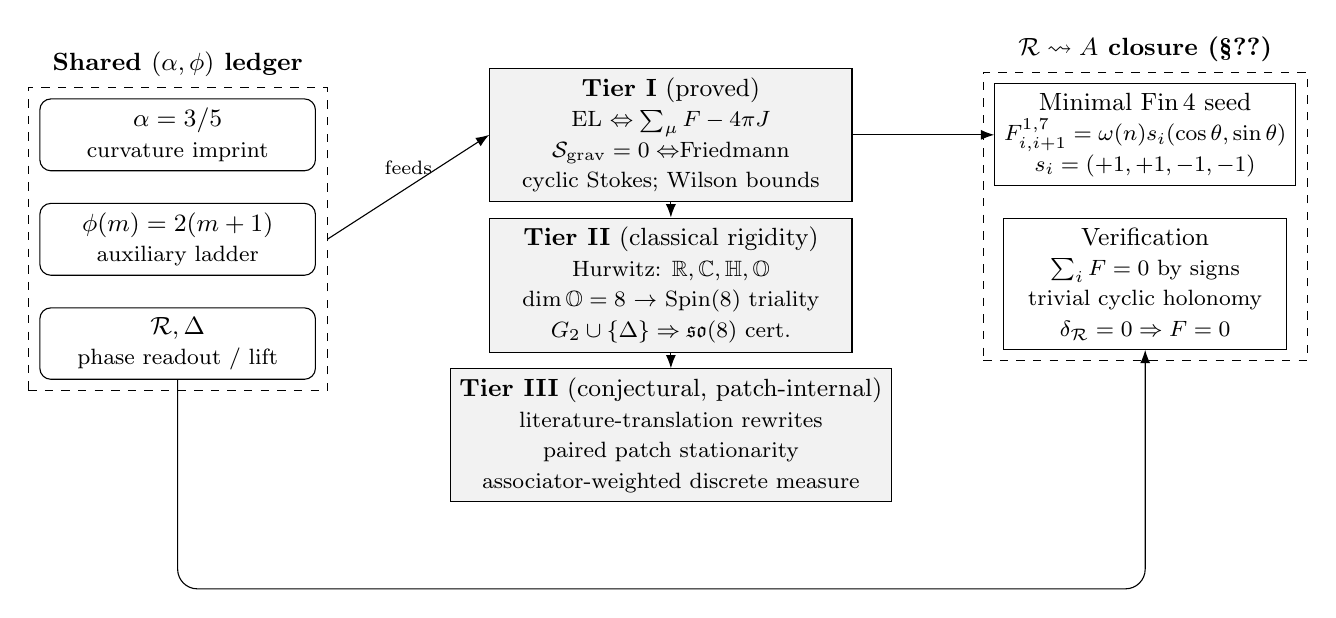
\begin{tikzpicture}[
  font=\small,
  >=Latex,
  node distance=4mm,
  arr/.style={->,rounded corners=2.5mm}
]
% --- left column: shared parameter ledger ---
\node[draw,rounded corners,align=center,minimum width=3.5cm] (alpha) {\(\alpha=3/5\)\\\footnotesize curvature imprint};
\node[draw,rounded corners,align=center,minimum width=3.5cm,below=of alpha] (phi) {\(\phi(m)=2(m+1)\)\\\footnotesize auxiliary ladder};
\node[draw,rounded corners,align=center,minimum width=3.5cm,below=of phi] (R) {\(\mathcal{R},\Delta\)\\\footnotesize phase readout / lift};
\node[fit=(alpha)(phi)(R),draw,dashed,inner sep=4pt,label=above:{\textbf{Shared \((\alpha,\phi)\) ledger}}] (ledger) {};
% --- middle: uniqueness tiers ---
\node[draw,fill=gray!10,align=center,minimum width=4.6cm,right=22mm of alpha] (T1) {\textbf{Tier I} (proved)\\\footnotesize EL \(\Leftrightarrow \sum_\mu F-4\pi J\)\\\footnotesize \(\mathcal{S}_{\mathrm{grav}}=0\Leftrightarrow\)Friedmann\\\footnotesize cyclic Stokes; Wilson bounds};
\node[draw,fill=gray!10,align=center,minimum width=4.6cm,below=2mm of T1] (T2) {\textbf{Tier II} (classical rigidity)\\\footnotesize Hurwitz: \(\mathbb{R},\mathbb{C},\mathbb{H},\mathbb{O}\)\\\footnotesize \(\dim\mathbb{O}=8\) \(\to\) Spin(8) triality\\\footnotesize \(G_2\cup\{\Delta\}\Rightarrow\mathfrak{so}(8)\) cert.};
\node[draw,fill=gray!10,align=center,minimum width=4.6cm,below=2mm of T2] (T3) {\textbf{Tier III} (conjectural, patch-internal)\\\footnotesize literature-translation rewrites\\\footnotesize paired patch stationarity\\\footnotesize associator-weighted discrete measure};
% --- right: minimal seed ---
\node[draw,align=center,minimum width=3.6cm,right=18mm of T1] (seed) {Minimal \(\mathrm{Fin}\,4\) seed\\\footnotesize \(F^{1,7}_{i,i+1}=\omega(n)s_i(\cos\theta,\sin\theta)\)\\\footnotesize \(s_i=(+1,+1,-1,-1)\)};
\node[draw,align=center,minimum width=3.6cm,below=of seed] (verif) {Verification\\\footnotesize \(\sum_i F=0\) by signs\\\footnotesize trivial cyclic holonomy\\\footnotesize \(\delta_{\mathcal{R}}=0\Rightarrow F=0\)};
\node[fit=(seed)(verif),draw,dashed,inner sep=4pt,label=above:{\textbf{\(\mathcal{R}\rightsquigarrow A\) closure (\S\ref{subsec:minimal-seed})}}] (rseed) {};
% --- routing channel below tier stack (ledger → verification) ---
\coordinate (underTiers) at ($(T3.south)+(0,-11mm)$);
% --- arrows ---
\draw[arr] (ledger.east) -- node[above,font=\scriptsize,yshift=1pt]{feeds} (T1.west);
\draw[arr] (T1) -- (T2);
\draw[arr] (T2) -- (T3);
\draw[arr] (R.south) -- (R.south |- underTiers) -- (underTiers -| verif.south) -- (verif.south);
\draw[arr] (T1.east) -- (seed.west);
\end{tikzpicture}
\caption{Executive summary. The shared \((\alpha,\phi)\) ledger forced by the predecessor papers feeds both the proved Tier-I dynamics (EL identity, Friedmann constraint, holonomy bounds) and the explicit minimal-cycle realization \(\mathcal{R}\rightsquigarrow A\). Tier~II is classical division-algebra rigidity plus the certified \(G_2\cup\{\Delta\}\Rightarrow\mathfrak{so}(8)\) closure; Tier~III is a patch-internal interoperability programme (literature-translation rewrites, paired patch stationarity, associator-weighted discrete measure)---\emph{not} a continuum-limit programme. Per the patch-theory reader contract above, no continuum limit is required for foundational validity.}
\label{fig:exec-summary}
\end{figure}

\subsection{Nomenclature}
\label{subsec:nomenclature}

For readers arriving from outside the HQIV programme, the symbols below recur throughout the text and are defined formally where they first appear (HQVM is fixed in Subsection~\ref{subsec:hqvm}):
\begin{description}[
  font=\normalfont,
  leftmargin=0pt,
  labelwidth=0pt,
  itemsep=0.45\baselineskip,
  parsep=0.1\baselineskip,
  topsep=0.25\baselineskip,
  style=nextline
]
  \item[HQVM]
  Horizon-Quantized Vacuum Metric: the non-FLRW homogeneous background, lapse, and Friedmann constraint sector defined in Subsection~\ref{subsec:hqvm}; not an independent acronym elsewhere in the series.
  \item[\(\mathrm{Fin}\,n\)]
  Finite index type \(\{0,1,\dots,n-1\}\); \(\mathrm{Fin}\,8\) labels octonion channels and \(\mathrm{Fin}\,4\) labels spacetime indices.
  \item[\(A^a{}_\mu\), \(F^a{}_{\mu\nu}\)]
  Discrete gauge potential and field strength on \(\mathrm{Fin}\,8\times\mathrm{Fin}\,4\); \(F^a{}_{\mu\nu}=A^a{}_\nu-A^a{}_\mu\).
  \item[\(m\)]
  Shell index, \(m\in\mathbb{N}\). Calibration shell is \(m_{\mathrm{ref}}=4\) (proton anchor in the QCD-onset ladder).
  \item[\(\rho\), \(K\), \(\Omega\)]
  Discrete densities on the null-shell ladder: weight, curvature numerator, and curvature ratio; \(\Omega_k(m;m_{\mathrm{ref}})\) is the partial curvature ratio at \(m\).
  \item[\(\mathcal{R}\)]
  Normalized cumulative phase readout; \(\delta_{\mathcal{R}}(n)=\mathcal{R}(n+1)-\mathcal{R}(n)\) is the per-shell increment.
  \item[\(\Delta\)]
  Phase-lift generator in the \((e_1,e_7)\) plane of the octonion units; \(\Delta\in\mathfrak{so}(8)\).
  \item[\(G_2\)]
  Automorphism Lie group of the octonions, \(\mathrm{Aut}(\mathbb{O})\). The notation \(G_2\cup\{\Delta\}\) means the linear span of \(G_2\) and \(\Delta\) under the bracket.
  \item[\(\alpha\), \(\gamma_{\mathrm{HQIV}}\)]
  Curvature imprint and unit-split coefficient; \(\alpha=3/5\), \(\gamma=2/5\); \((3-\gamma_{\mathrm{HQIV}})=13/5\) is the Friedmann prefactor.
  \item[\(\phi(m)\)]
  Auxiliary scalar on the temperature ladder, \(\phi(m)=2(m+1)\); also \(\phi_{\mathrm{val}}\) as an action-cell parameter.
  \item[\(G_{\mathrm{eff}}(\phi)\)]
  Effective gravitational coupling \(\phi^{\alpha}\) in the HQVM Friedmann identity.
  \item[\(\mathcal{S}_O\), \(\mathcal{S}_{\mathrm{grav}}\), \(\mathcal{S}_{\mathrm{tot}}\)]
  O--Maxwell, gravity, and total action cells (Definition~\ref{def:total}).
  \item[\(v_{\mathrm{lockin}}\)]
  Lock-in vev proxy in the weak/Higgs scaffold,
  \(v_{\mathrm{lockin}}=\sqrt{\eta_{\mathrm{paper}}\,\Omega_k(m_{\mathrm{lockin}};m_{\mathrm{lockin}})}\).
\end{description}

\subsection{HQVM backbone}
\label{subsec:hqvm}

HQIV replaces a homogeneous FLRW ansatz with a \emph{patch} background tied to horizon readouts.
The \textbf{Horizon-Quantized Vacuum Metric} (HQVM) is the name of that background sector in synchronous-comoving gauge (vanishing shift).

\begin{definition}[HQVM metric and lapse]
\label{def:hqvm}
In the HQVM chart used throughout the HQIV library \cite{ettinger2026hqiv,hqiv-lean}, the ADM lapse is
\[
  N(\Phi,\phi,t) \;=\; 1 + \Phi + \frac{\phi\,t}{c},
\]
where \(\Phi\) is the Newtonian potential slot, \(t\) is coordinate time, \(c\) is the speed of light, and \(\phi\) is the \emph{same} auxiliary scalar that enters the temperature ladder \(\phi(m)=2(m+1)\) and the O--Maxwell \(\phi\)-coupling (the \hyperref[lean:phi-ladder]{auxiliary field ladder} and \hyperref[lean:lapse-bridge]{lapse-dragging bridge}).
The spatial part is carried by a synchronous diagonal metric on \(\mathrm{Fin}\,4\) with scale factor and curvature imprint data fixed by the discrete null-lattice spine; the load-bearing statement for cosmology in this paper is not a continuum line element but the \textbf{HQVM Friedmann identity} obtained when the gravitational action cell \(\mathcal{S}_{\mathrm{grav}}\) vanishes (Theorem~\ref{thm:friedmann}).
\end{definition}

\begin{definition}[HQVM octonionic seed]
\label{def:hqvm-seed}
The phrase \emph{HQVM octonionic seed} means the explicit \(\mathrm{Fin}\,8\) matrix carrier fixed in \cite{hqiv-so8-paper}: Fano-table left multiplications \(L(e_a)\), the phase-lift \(\Delta\) in the \((e_1,e_7)\) plane, and the certified Lie closure \(G_2\cup\{\Delta\}\Rightarrow\mathfrak{so}(8)\).
Gauge potentials \(A^a{}_\mu\) in this manuscript are octonion-indexed fields on the same carrier; they are not an extra postulate beyond that seed.
\end{definition}

\begin{remark}[Effective coupling and homogeneous calibration]
\label{rem:hqvm-coupling}
On the homogeneous branch, the effective gravitational coupling is \(G_{\mathrm{eff}}(\phi)=\phi^{\alpha}\) with the forced imprint \(\alpha=3/5\) (the \hyperref[lean:imprint-alpha]{curvature imprint \(\alpha=3/5\)}).
Identifying the Hubble slot with \(\phi\) in that sector is the HQVM calibration carried by the \hyperref[lean:lapse-bridge]{lapse-dragging cross-sector identification}; it threads the same \(\phi\) into \(\mathcal{L}_\phi\), into \(N\), and into the Friedmann constraint~\eqref{eq:hqvm-friedmann-explicit} without introducing a separate dark-energy knob.
\end{remark}

\section{Logical placement and reader contract}
\label{sec:placement}

\subsection{Predecessors}

\cite{hqiv-so8-paper} gives the chain
\[
\text{uniform growth} \Longrightarrow K \Longrightarrow \Omega \Longrightarrow \mathcal{R}
\Longrightarrow \Delta \Longrightarrow \langle G_2,\Delta\rangle_{\mathrm{Lie}}=\mathfrak{so}(8)
\]
under explicit imports (quadratic shell law, \(\alpha=3/5\) normalization story, Fano octonion model, \((e_1,e_7)\) plane). \cite{hqiv-3d-growth-paper} isolates the quadratic-versus-cubic dimensional hinge in \(3{+}1\), records the conditional forcing theorem (a shared-manifold rapidity bridge plus the imported \(\mathfrak{so}(8)\) span witness conclude common rapidity, curvature positivity/divergence, reference normalization, and the span witness), and develops the Hurwitz/triality narrative with careful scope.

\subsection{Where this paper sits in the three-layer stack}

It is useful to picture HQIV formalization as three layers that \emph{compose} in the repository narrative but have different logical strengths. The \textbf{discrete growth layer} (shell counts, \(K,\Omega,\mathcal{R}\), lattice--\(\alpha\) coherence) is the strongest combinatorial spine; the \textbf{Lie closure layer} (\(G_2\cup\{\Delta\}\Rightarrow\mathfrak{so}(8)\) on explicit matrices) is a certified linear-algebra certificate once seeds are fixed; the \textbf{variational layer} of the present manuscript packages equations of motion and constraints as stationarity of explicit functionals over the same octonion-indexed cutoff. This paper does \emph{not} merge those layers into a single implication from poset axioms; it documents the third layer precisely and explains how it is designed to interoperate with the first two through shared parameters \((\alpha,\phi)\).

\subsection{What this paper adds}
\label{subsec:adds}

\begin{itemize}
\item \textbf{Discrete O--Maxwell action and EL identities} (Sect.~\ref{sec:discrete}): the \hyperref[lean:F-from-A]{discrete field strength}, the \hyperref[lean:LO-kinetic]{three additive density pieces}, the \hyperref[lean:LO-Maxwell]{full O--Maxwell density and action cell}, the \hyperref[lean:EL-divergence]{discrete EL identity}, and the \hyperref[lean:add-J]{source superposition correction}.
\item \textbf{Gravity constraint and total action} (Sect.~\ref{sec:grav}): the \hyperref[lean:S-grav]{gravitational constraint as Friedmann}, the \hyperref[lean:total-action]{total action and joint EL/Friedmann packaging}, and the lapse-dragging cross-sector identification (\hyperref[lean:lapse-bridge]{shared \(\phi\) and \(\alpha\) across O--Maxwell and GR}).
\item \textbf{Holonomy alignment on the same \(F\) slots} (Sect.~\ref{sec:holonomy}): the \hyperref[lean:cyclic-flux]{discrete Stokes identity}, the \hyperref[lean:trivial-holonomy]{trivial cyclic plaquette holonomy}, and the \hyperref[lean:wilson-bounds]{two-sided Wilson bound on the kinetic aggregate}.
\item \textbf{Minimal readout-to-gauge seed on the \(\mathrm{Fin}\,4\) cycle} (Sect.~\ref{sec:bridge}): the \hyperref[lean:readout-seed]{minimal seed} \(\mathcal{R}\rightsquigarrow A\) on the smallest spacetime cycle, certified Stokes-compatible.
\item \textbf{Weak/Higgs Tier-III scaffold on top of the proved abelian core} (Sect.~\ref{sec:weak-higgs-scaffold}): the \hyperref[lean:weakHiggs-scaffold]{typed extension surface}, with theorem-level reductions back to the proved abelian action when extension slots are switched off.
\end{itemize}

\subsection{Scope and not claimed}
\label{subsec:not-claimed}

\begin{itemize}
\item Causal poset axioms \emph{alone} do not imply this action; the quadratic shell law, octonion table, and plane choices remain explicit imports where used.
\item No continuum path integral, path-integral anomaly measure, or uniqueness of measure is proved here, and none is required for the discrete core claims of this paper. Finite SM anomaly-trace cancellation and patch topological-sector discharge are proved upstream (\leanfile{Hqiv/Algebra/AnomalyCancellation.lean}, \leanfile{Hqiv/QuantumMechanics/PatchTopologicalObstruction.lean}; see the patch-theory reader contract above).
\item No claim that alternative discrete variational ans\"atze cannot be written off the HQIV design path; Tier~I uniqueness is \emph{internal} to the stated Lagrangian class.
\item The patch-internal bridge \(\mathcal{R}\rightsquigarrow A\) with bookkeeping on enlarged discrete patches is deferred to the \hyperref[lean:scaffold-bridge]{manifold-Lagrangian scaffold and lattice/continuum coincidence interface} (Sect.~\ref{sec:bridge}); the explicit minimal seed of Subsection~\ref{subsec:minimal-seed} is the first discrete closure on one plaquette.
\item \textbf{Tier III is \emph{not} a continuum-limit programme.} Per the patch-theory reader contract above, the discrete patch layer is the ontology and several Tier-I results would be erased rather than refined by an ultraviolet/mesh continuum limit; whenever Tier III refers to ``translation'' or ``coincidence'' with continuum notation, that translation is a calculation-approximation rewrite for cross-citation only, not an underlying theory of which HQIV is a discretization. The detailed scope is fixed in Subsection~\ref{subsec:tierIII}.
\end{itemize}

\section{Discrete O--Maxwell action}
\label{sec:discrete}

Fix octonion channel index \(a\in \mathrm{Fin}\,8\) and spacetime index \(\mu,\nu\in \mathrm{Fin}\,4\) as in the library.

\begin{definition}[\texorpdfstring{\hyperref[lean:F-from-A]{Discrete field strength}}{Discrete field strength}]
\label{def:F}
For \(A : \mathrm{Fin}\,8 \to \mathrm{Fin}\,4 \to \mathbb{R}\),
\[
F^a{}_{\mu\nu}(A) := A^a{}_\nu - A^a{}_\mu .
\]
\end{definition}

\begin{definition}[Kinetic and source densities]
\label{def:kinetic-source}
The kinetic aggregate (\hyperref[lean:LO-kinetic]{kinetic density}) is
\begin{equation}
\label{eq:Lkin-expanded}
\mathcal{L}_{\mathrm{kin}}(A)
:= -\frac14 \sum_{a\in \mathrm{Fin}\,8}\;\sum_{\mu,\nu\in \mathrm{Fin}\,4}
\frac{\bigl(F^a{}_{\mu\nu}(A)\bigr)^2}{2}.
\end{equation}
The factor \(\tfrac12\) inside the sum implements antisymmetric bookkeeping while summing over all ordered pairs \((\mu,\nu)\). The source interaction for \(J_{\mathrm{src}} : \mathrm{Fin}\,8 \to \mathrm{Fin}\,4 \to \mathbb{R}\) is
\begin{equation}
\label{eq:Lsource-expanded}
\mathcal{L}_{\mathrm{src}}(J_{\mathrm{src}},A)
:= \sum_{a\in \mathrm{Fin}\,8}\;\sum_{\nu\in \mathrm{Fin}\,4} (J_{\mathrm{src}})^a{}_\nu\, A^a{}_\nu .
\end{equation}
\end{definition}

\begin{definition}[\texorpdfstring{\hyperref[lean:LO-Maxwell]{Full O--Maxwell density and action cell}}{Full O-Maxwell density and action cell}]
\label{def:LOmaxwell}
For \(\phi_{\mathrm{val}}>-1\), the \(\phi\)-coupling term is
\[
\mathcal{L}_\phi(A,\phi_{\mathrm{val}})
:= \alpha\,\log(\phi_{\mathrm{val}}+1)\sum_{\nu\in \mathrm{Fin}\,4} (\mathrm{grad}_\phi)_\nu\, A^0{}_\nu ,
\]
where \((\mathrm{grad}_\phi)_\nu\) is the \(\phi\)-gradient slot (currently a zero placeholder in the action module; continuum gradients live in the modified-Maxwell module---see Remark~\ref{rem:modified-maxwell}). The full density is
\[
\mathcal{L}_O[J_{\mathrm{src}}](A,\phi_{\mathrm{val}})
:= \mathcal{L}_{\mathrm{kin}}(A) + 4\pi\,\mathcal{L}_{\mathrm{src}}(J_{\mathrm{src}},A) + \mathcal{L}_\phi(A,\phi_{\mathrm{val}}),
\]
and the \emph{action cell} is the same real number.
\end{definition}

\begin{theorem}[\texorpdfstring{\hyperref[lean:EL-divergence]{Discrete Euler--Lagrange matches divergence of \(F\) minus sources}}{Discrete Euler-Lagrange matches divergence of F minus sources}]
\label{thm:EL}
For source \(J_{\mathrm{src}}\), potential \(A\), and scalar \(\phi_{\mathrm{val}}\) with \(\phi_{\mathrm{val}}+1>0\), the EL covector at \((a,\nu)\) equals
\[
\sum_{\mu\in \mathrm{Fin}\,4} F^a{}_{\mu\nu}(A) - 4\pi (J_{\mathrm{src}})^a{}_\nu
-\begin{cases}
\alpha\,\log(\phi_{\mathrm{val}}+1)\,(\mathrm{grad}_\phi)_\nu, & a=0,\\
0, & a\neq 0 .
\end{cases}
\]
\end{theorem}

\begin{proof}[Sketch (conceptual; the Lean proof is definitional/rewrite)]
Vary \(A^b{}_\sigma\to A^b{}_\sigma+\varepsilon\,\delta^b_a\,\delta^\sigma_\nu\) in \(\mathcal{L}_{\mathrm{kin}}\). Each \(F^b{}_{\mu\sigma}\) shifts by \(\varepsilon(\delta^\mu_\sigma-\delta^\mu_\nu)\) when \(\sigma=\nu\), and each \(F^b{}_{\nu\mu}\) shifts by the opposite increment. Collecting coefficients of \(\varepsilon\) produces a telescoping sum over \(\mu\) that yields \(\sum_\mu F^a{}_{\mu\nu}\)---the discrete analogue of \(\partial_\mu F^{\mu\nu}\). The source term \(4\pi J\!\cdot\!A\) contributes \(-4\pi J^a{}_\nu\) to the EL covector, and the \(\phi\)-coupling contributes only on channel \(a=0\) by construction. This is the standard polynomial-gauge calculation carried out on the finite index set.
\end{proof}

\begin{remark}[The shared parameter ledger \((\alpha,\gamma)\) and the auxiliary-field ladder]
The imprint \(\alpha=3/5\) entering \(\mathcal{L}_\phi\) is the \emph{same} rational identity forced by the discrete light-cone in the predecessor papers (\hyperref[lean:imprint-alpha]{curvature imprint \(\alpha=3/5\)}); readers who want the thermodynamic packaging (Jacobson/Brodie on horizons, monogamy template) should consult the thermodynamic-derivation appendix of \cite{hqiv-3d-growth-paper}. The auxiliary scalar follows the temperature ladder \(\phi(m)=2(m+1)\) (\hyperref[lean:phi-ladder]{auxiliary field ladder}). On the gravity side, the unit-split coefficient \((3-\gamma_{\mathrm{HQIV}})=13/5\) enters the Friedmann constraint as a fixed rational prefactor (Theorem~\ref{thm:friedmann}). Thus the \((\alpha,\gamma)\) pair is simultaneously the monogamy/unit-split pair from the growth papers and the coupling/normalization pair threading the action, the HQVM metric, and the auxiliary field.
\end{remark}

\begin{remark}[Relation to the emergent inhomogeneous Maxwell equation]
\label{rem:modified-maxwell}
The modified-Maxwell module packages the same \(-4\pi J_{\mathrm{src}}\) source slot and \(\alpha\)-weighted \(\phi\)-gradient correction as Theorem~\ref{thm:EL} (\hyperref[lean:emergent-maxwell]{emergent inhomogeneous Maxwell slot}). The discrete EL above uses an explicit \(\sum_\mu F\) surrogate, while the emergent file still carries a placeholder for the covariant divergence term; the maintained design contract is \emph{source-slot alignment} between the EL and the emergent inhomogeneous equation. Completing the identification requires wiring the same continuum-gradient components into both sides, a task already in progress in the continuum-O-Maxwell-closure module.
\end{remark}

\section{Gravitational sector and total action}
\label{sec:grav}

\begin{theorem}[\texorpdfstring{\hyperref[lean:S-grav]{Gravitational constraint equals Friedmann}}{Gravitational constraint equals Friedmann}]
\label{thm:friedmann}
The HQVM gravitational action \(\mathcal{S}_{\mathrm{grav}}(\phi,\rho_m,\rho_r)\) vanishes if and only if the HQVM Friedmann identity holds at \((\phi,\rho_m,\rho_r)\). For \(\phi\ge 0\) the constraint is equivalent to the explicit rational form
\[
\frac{13}{5}\,\phi^2 \;=\; 8\pi\,\phi^{\alpha}\,(\rho_m+\rho_r),
\qquad \alpha=\frac35.
\]
\end{theorem}

\begin{definition}[\texorpdfstring{\hyperref[lean:total-action]{Total action} and \hyperref[lean:add-J]{current superposition}}{Total action and current superposition}]
\label{def:total}
Write \(\mathcal{S}_O[J_{\mathrm{src}}](A,\phi_{\mathrm{val}}):=\mathcal{L}_O[J_{\mathrm{src}}](A,\phi_{\mathrm{val}})\) for the O--Maxwell cell and let \(\mathcal{S}_{\mathrm{grav}}(\phi,\rho_m,\rho_r)\) denote the HQVM gravity action of Theorem~\ref{thm:friedmann}. The total cell is
\[
\mathcal{S}_{\mathrm{tot}}[J_{\mathrm{src}}](A,\phi,\rho_m,\rho_r)
:= \mathcal{S}_O[J_{\mathrm{src}}](A,\phi) + \mathcal{S}_{\mathrm{grav}}(\phi,\rho_m,\rho_r) .
\]
For two sources, the source-superposition identity reads
\begin{multline}
\label{eq:superposition-correction}
\mathcal{S}_{\mathrm{tot}}[J_1+J_2](A,\phi,\rho_m,\rho_r)
= \mathcal{S}_{\mathrm{tot}}[J_1](A,\phi,\rho_m,\rho_r)
+ \mathcal{S}_{\mathrm{tot}}[J_2](A,\phi,\rho_m,\rho_r) \\
{}- \mathcal{L}_{\mathrm{kin}}(A) - \mathcal{L}_\phi(A,\phi) - \mathcal{S}_{\mathrm{grav}}(\phi,\rho_m,\rho_r).
\end{multline}
The O--Maxwell part alone satisfies the simpler linearity in \(J\) only for the \(4\pi\,J\!\cdot\!A\) piece; the kinetic and \(\phi\) terms are shared, so naive addition of two full densities double-counts those shared blocks.
\end{definition}

\begin{example}[Flat potential, trivial current, balanced densities]
\label{ex:simultaneous}
Take \(A^a{}_\mu\equiv 0\) so \(F^a{}_{\mu\nu}=0\) and \(\mathcal{L}_{\mathrm{kin}}=0\); take the canonical current \(J_O\equiv 0\) so \(\mathcal{L}_{\mathrm{src}}=0\); take the \(\phi\)-gradient slot to vanish so \(\mathcal{L}_\phi=0\). Then \(\mathcal{S}_O=0\). Choose \(\phi=1\) (Hubble reference in natural units). The Friedmann constraint \((13/5)\phi^2 = 8\pi\,\phi^{\alpha}(\rho_m+\rho_r)\) with \(\alpha=3/5\) gives \(\rho_m+\rho_r = 13/(40\pi)\). For these values \(\mathcal{S}_{\mathrm{grav}}=0\) and the EL covector reduces to \(\sum_\mu F=0\), which holds trivially. This is the same decoupled ``zero sector'' used to illustrate the joint EL/Friedmann packaging (\hyperref[lean:total-action]{total action and joint EL/Friedmann packaging}): gravity is a constraint on \((\phi,\rho)\); gauge EL is a separate stationarity problem in \(A\) once \(J\) and \(\phi\) data are fixed.
\end{example}

\begin{remark}[\texorpdfstring{Lapse dragging, lapse-corrected GR, and the demystified $\Lambda$}{Lapse dragging, lapse-corrected GR, and demystified Lambda}]
\label{rem:lapse-lambda}
The constraint \(\mathcal{S}_{\mathrm{grav}}=0\) of Theorem~\ref{thm:friedmann} is \emph{not} the textbook flat FLRW equation of Einstein GR with a fundamental cosmological constant \(\Lambda\),
\[
H^2=\frac{8\pi G}{3}\,\rho_{\mathrm{tot}}+\frac{\Lambda c^2}{3}.
\]
Instead, for \(\phi\ge 0\), the HQVM Friedmann identity is the explicit rational form
\begin{equation}
\label{eq:hqvm-friedmann-explicit}
\frac{13}{5}\,\phi^2 = 8\pi\,G_{\mathrm{eff}}(\phi)\,(\rho_m+\rho_r),
\qquad G_{\mathrm{eff}}(\phi)=\phi^{\alpha},\quad \alpha=\frac35,
\end{equation}
where \((3-\gamma_{\mathrm{HQIV}})=13/5\) is the unit-split/monogamy coefficient. There is therefore \textbf{no independent \(\Lambda\) knob}: whatever plays the role of a ``dark'' constant term in a standard frame is packaged here into the \(\phi\)-dependent coupling \(G_{\mathrm{eff}}\) and the fixed rational prefactor inherited from the same \((\alpha,\gamma)\) ledger that the thermodynamic appendix of \cite{hqiv-3d-growth-paper} derives from Jacobson/Brodie horizon bookkeeping. In the HQVM narrative, \(\phi\) is the relative-observer energy normalizer (auxiliary field / temperature ladder), not an ad hoc fifth force; identifying \(H\) with \(\phi\) in the homogeneous sector is the calibration carried by the \hyperref[lean:lapse-bridge]{lapse-dragging cross-sector identification}. The minimal seed of Subsection~\ref{subsec:minimal-seed} makes the coupling explicit at the variational level: the same readout increments and \(\log(\phi+1)\) weighting that thread into \(\mathcal{L}_\phi\) also enter the gravitational constraint through \(\phi\) and \(\alpha\). A Tier~III continuum limit would target Einstein-type dynamics with an \emph{emergent}, normalization-sensitive effective vacuum contribution---not a fitted fundamental \(\Lambda\).

\medskip
\noindent\textbf{Lapse dragging.}
In synchronous-comoving gauge the HQVM lapse is \(N=1+\Phi+\phi t/c\). Following \cite{jacobson1995,brodie2026}, we use the term \emph{lapse dragging} for the coupling of the cumulative horizon phase \(\phi t/c\) to proper time \emph{and} to the same \(\phi\) slot that appears in \(\mathcal{L}_\phi\) and in~\eqref{eq:hqvm-friedmann-explicit}. The identification of that slot across the O--Maxwell and homogeneous GR branches, together with the matching of the imprint exponent \(\alpha\) on both sides, is the content of the \hyperref[lean:lapse-bridge]{lapse-dragging cross-sector identification}. Thus ``lapse dragging'' is not an extra postulate: it is the visible name for the shared \(\phi\) morphism already audited inside the variational layer.

\begin{table}[ht]
\centering
\small
\caption{Effective gravitational coupling in natural units (\(G_0=1\)): \(G_{\mathrm{eff}}(\phi)/G_0=\phi^{3/5}\) (rounded).}
\label{tab:Geff-numerics}
\begin{tabular}{@{}c@{\quad}c@{}}
\hline
\(\phi\) & \(G_{\mathrm{eff}}(\phi)/G_0=\phi^{3/5}\) \\
\hline
\(0.5\) & \(0.660\) \\
\(0.8\) & \(0.875\) \\
\(1.0\) & \(1.000\) \\
\(1.2\) & \(1.116\) \\
\(1.5\) & \(1.275\) \\
\(2.0\) & \(1.516\) \\
\hline
\end{tabular}
\end{table}

\medskip
\noindent\textbf{Galactic rotation curves (first-pass SPARC-style sanity check, not a Tier-I claim).}
Flat disk kinematics in the low-acceleration regime are a standard testbed for modified-inertia ideas derived from horizon overlap \cite{brodie2026}, and the SPARC database \cite{lelli2016sparc} has become the reference observational input for such fits. The same \(\alpha=3/5\) that enters \(G_{\mathrm{eff}}(\phi)=\phi^{\alpha}\) and \(\mathcal{L}_\phi\) is the imprint forced by the discrete light-cone layer (\hyperref[lean:imprint-alpha]{curvature imprint \(\alpha=3/5\)}); the \emph{conjectural} packaging is that a running \(G_{\mathrm{eff}}\) tied to \(\phi\) and a Brodie-type inertia factor \(f(a_{\mathrm{loc}},\phi)\) are two faces of one horizon bookkeeping constraint at different kinematic scales. Rather than only assert this, we compute. Table~\ref{tab:sparc-firstpass} reports a first-pass numerical check produced by the companion HQIV galaxy-rotation calculator \cite{hqiv-orbital}, which uses the same \(\alpha=3/5\) inertia factor \(f(a_{\mathrm{loc}},\phi)=a_{\mathrm{loc}}/(a_{\mathrm{loc}}+\phi/6)\) and the angular Rindler denominator \(D_R=1+(\gamma_{\mathrm{HQIV}}/2)(c/v)^{2}\) used in the flyby paper, applied to a single-exponential baryonic disk for six SPARC-scale spirals. \emph{No fitting parameters were tuned}: each row uses the literature stellar mass and disk scale length as the only inputs; the predicted circular speed at the reference radius is read off without any continuum limit, dark-matter halo, or per-galaxy adjustment. With those inputs the predicted speed at the reference radius lies within roughly \(\pm 20\%\) of the observed flat-curve value for the five disk-dominated spirals (M33, NGC 2403, NGC 3198, NGC 6503, UGC 2885), with the gas-dominated dwarf DDO 154 (where the single-exponential disk is acknowledged to be a crude stand-in) as the expected outlier. This is a sanity check that the variational layer's \(\alpha\)-coupling is in the right ballpark when stress-tested against rotation-curve scales; a full SPARC mass-model import (HI plus bulge plus disk components, per-galaxy distance and inclination uncertainties, joint \(\chi^{2}\) marginalization over the \(\phi\)-shell index) is deferred to a dedicated Tier-III companion paper.
\end{remark}

\begin{table}[ht]
\centering
\renewcommand{\arraystretch}{1.18}
\caption{First-pass SPARC-style sanity check of the HQIV \(\alpha=3/5\) inertia factor on six exponential-disk presets, computed by \texttt{hqiv\_galaxy\_rotation.py} \cite{hqiv-orbital}. The Newtonian baryonic prediction at the reference radius is shown alongside the HQIV prediction (single-exponential disk, no halo, no fit parameters); residuals are \((v_{\mathrm{HQIV}}-v_{\mathrm{obs}})/v_{\mathrm{obs}}\). The HQIV calculator is the same module used in the flyby paper and reuses \(f(a,\phi)=a/(a+\phi/6)\) plus the angular Rindler denominator without modification. DDO 154 (gas-dominated dwarf) is the expected outlier: the exponential-disk approximation is crude there. A full SPARC fit is a Tier-III companion task. The exact run that produced this table ships in the supplementary script bundle (Appendix~\ref{app:scripts}, file \texttt{sparc\_firstpass\_table.py}).}
\label{tab:sparc-firstpass}
\begin{tabular}{lcccccc}
\hline
Galaxy & \(M_\mathrm{disk}\) (\(M_\odot\)) & \(R_d\) (kpc) & \(r_{\mathrm{ref}}\) (kpc) & \(v_\mathrm{bary}\) (km/s) & \(v_\mathrm{HQIV}\) (km/s) & \(v_\mathrm{obs}\) (km/s) \\
\hline
M33      & \(5{\times}10^{9}\)   & 1.8 & 10 & 45.8  & 113.0 & 110 \\
NGC 2403 & \(1{\times}10^{10}\)  & 1.8 & 12 & 59.6  & 120.4 & 135 \\
NGC 3198 & \(5{\times}10^{10}\)  & 3.5 & 20 & 102.5 & 177.1 & 150 \\
NGC 6503 & \(6{\times}10^{9}\)   & 1.7 & 8  & 55.3  & 113.5 & 115 \\
DDO 154\(^{\dagger}\) & \(5{\times}10^{8}\) & 1.6 & 8  & 16.1  & 97.9  & 50  \\
UGC 2885 & \(2{\times}10^{11}\)  & 8.0 & 40 & 143.7 & 259.4 & 300 \\
\hline
\multicolumn{7}{l}{\footnotesize\(^{\dagger}\)Gas-dominated dwarf; single-exponential disk acknowledged to be a crude stand-in.}
\end{tabular}
\end{table}

\begin{remark}[Superposition discipline]
\label{rem:superposition}
Physically, adding two current systems \(J_1+J_2\) should increase only the interaction energy \(\int J\!\cdot\!A\) (here, the discrete \(4\pi\,J\!\cdot\!A\) term) while retaining a \emph{single} copy of the gauge-field self-energy and a \emph{single} Friedmann constraint for the shared \((\phi,\rho)\). Equation~\eqref{eq:superposition-correction} is the bookkeeping correction that enforces ``no double counting'' of \(\mathcal{L}_{\mathrm{kin}}\), \(\mathcal{L}_\phi\), and \(\mathcal{S}_{\mathrm{grav}}\) when concatenating two source packages into one variational cell. This matches the broader HQIV audit discipline: only book-kept morphisms count as physical intermediates.
\end{remark}

\begin{remark}[Joint EL/Friedmann packaging]
The \hyperref[lean:total-action]{total action and joint EL/Friedmann packaging} records the joint pattern: Friedmann arises as the gravitational constraint, while the gauge sector's EL identities are the discrete equations of motion at the chosen potential.
\end{remark}

\section{Holonomy alignment and the same \texorpdfstring{$F$}{F} data}
\label{sec:holonomy}

\subsection{Cyclic Stokes and trivial plaquette holonomy}

\begin{lemma}[\texorpdfstring{\hyperref[lean:cyclic-flux]{Cyclic flux sum}}{Cyclic flux sum}]
\label{lem:stokes}
For every channel \(a\) and every potential \(A\),
\[
\sum_{i\in \mathrm{Fin}\,4} F^a{}_{i,\,i+1}(A) = 0 .
\]
\end{lemma}

\paragraph{Expository telescoping.}
Unfold \(F^a{}_{i,i+1}=A^a{}_{i+1}-A^a{}_i\) for \(i=0,1,2,3\) on the cyclic \(\mathrm{Fin}\,4\) line, with \(3+1=0\) in the index ring. The sum is
\[
(A^a_1{-}A^a_0)+(A^a_2{-}A^a_1)+(A^a_3{-}A^a_2)+(A^a_0{-}A^a_3)=0,
\]
purely by cancellation; no input from octonion multiplication is used---only the abelian group structure of \(\mathbb{R}\) under addition. This is the discrete face of Stokes' theorem on the minimal spacetime cycle at the cutoff.

\begin{lemma}[\texorpdfstring{\hyperref[lean:trivial-holonomy]{Trivial abelian holonomy on the cycle}}{Trivial abelian holonomy on the cycle}]
\label{lem:hol-one}
With edge transports given by translation on \(\mathbb{R}\), \(\delta\mapsto (x\mapsto x+\delta)\), the cyclic plaquette holonomy built from the edges \(F^a{}_{i,i+1}\) equals the identity.
\end{lemma}

\begin{lemma}[\texorpdfstring{\hyperref[lean:wilson-bounds]{Kinetic vs.\ cyclic Wilson squares}}{Kinetic vs. cyclic Wilson squares}]
\label{lem:wilson-bounds}
For any \(x\in\mathbb{R}\),
\[
-\frac12 \sum_{a,i} \bigl((U^a_i x-x)^2\bigr)
\;\le\; \mathcal{L}_{\mathrm{kin}}(A)
\;\le\; -\frac14 \sum_{a,i} \bigl((U^a_i x-x)^2\bigr),
\]
where each \(U^a_i\) is translation on \(\mathbb{R}\) by the edge flux \(F^a{}_{i,i+1}\). Thus the global variational kinetic is bounded above and below by sums of squared abelian Wilson defects on the cyclic edges.
\end{lemma}

\begin{table}[ht]
\caption{Variational vs.\ holonomy reading of the same \(F\) slots.}
\label{tab:two-views}
\centering
\small
\begin{tabular}{@{}p{2.4cm}p{3.5cm}p{3.4cm}p{3.6cm}@{}}
\hline
Quantity & Variational meaning & Holonomy meaning & Reader-friendly anchor \\
\hline
\(F^a{}_{\mu\nu}\) & Kinetic density \(-\tfrac14 F^2\) summed over all \((\mu,\nu)\) & Edge flux for abelian transport & \hyperref[lean:F-from-A]{discrete field strength} \\
\(\sum_i F^a{}_{i,i+1}\) & Implied constraint on cyclic subset of pairs & Discrete Stokes: vanishing sum around cycle & \hyperref[lean:cyclic-flux]{discrete Stokes identity} \\
\(\prod_i U^a_i\) & (not used directly in \(\mathcal{L}\)) & Identity holonomy on closed plaquette & \hyperref[lean:trivial-holonomy]{trivial cyclic holonomy} \\
\(\mathcal{L}_{\mathrm{kin}}\) & Global \(8\times 4\times 4\) aggregate & Bounded by cyclic Wilson squares & \hyperref[lean:wilson-bounds]{two-sided Wilson bound} \\
\hline
\end{tabular}
\end{table}

\begin{remark}[\texorpdfstring{$\mathrm{SO}(8)$ action as internal wave-function transport}{SO8 wave-function transport}]
\label{rem:so8-wavefunction}
The \(\mathfrak{so}(8)\) generators that realize the certified \(G_2\cup\{\Delta\}\) closure act on the octonion-indexed components of the gauge potential \(A^a{}_\mu\) (\(a\in \mathrm{Fin}\,8\)) precisely as infinitesimal rotations of an \(8\)-component internal ``wave function.'' Left-multiplication by the imaginary units supplies the skew-adjoint operators \(L(e_i)\in\mathfrak{so}(8)\) that rotate one octonion direction into another while preserving the Euclidean norm on the carrier. The phase-lift generator \(\Delta\) then appears as a distinguished \(\mathrm{U}(1)\)-like rotation inside this larger structure, consistent with the normalized cumulative phase readout \(\mathcal{R}\) of \cite{hqiv-so8-paper}. In this reading the abelian plaquette transports of Lemma~\ref{lem:hol-one} are literally parallel-transport operators for the internal wave function along the minimal \(\mathrm{Fin}\,4\) cycle. The interpretation is motivational and does not modify any Lean-proved statement; it simply renders manifest why the eight-dimensional normed division algebra is the natural carrier once phase information and curvature are already present in the HQIV pipeline.
\end{remark}

\paragraph{Physical interpretation.}
The HQIV null-shell law is quadratic in the shell index while coarse spatial ball counting is cubic \cite{hqiv-3d-growth-paper}; the curvature channel built on that law feeds \(\alpha\) and hence both monogamy bookkeeping and the variational \(\phi\)-coupling (Remark in Sect.~\ref{sec:discrete}). Table~\ref{tab:two-views} makes the parallel explicit at the \emph{field} level: the same discrete \(F\) enters a global variational kinetic and a local Wilson/Stokes picture, so coercive control on plaquette defects is inherited from the same object that defines the action---the signature that the cutoff is not an arbitrary bookkeeping choice split across modules.

\paragraph{Non-abelian upgrade (pointer).}
Matrix-valued transports for the same combinatorial cycle are packaged separately as the \hyperref[lean:non-abelian-pointer]{non-abelian holonomy pointer}; the glue lemmas above stay in the abelian \(\mathbb{R}\) sector to isolate the discrete Stokes identity.

\subsection{Worked numerical example: minimal seed at \texorpdfstring{$m_{\mathrm{ref}}=4$}{m\_ref=4}}
\label{subsec:worked-example}

To make the kinetic / Wilson / EL bookkeeping concrete, fix the canonical seed of Subsection~\ref{subsec:minimal-seed} (sign pattern \(s=(+1,+1,-1,-1)\), unit vector \(v\) at angle \(\theta=\pi/4\) in the \((e_1,e_7)\) plane) at the calibration shell \(m_{\mathrm{ref}}=4\), and pick a small non-zero readout increment \(\delta_{\mathcal{R}}=10^{-2}\) for illustration.\footnote{Every numerical value in this subsection is reproduced byte-for-byte by the supplementary script \texttt{worked\_example\_minimal\_seed.py} in the bundle described in Appendix~\ref{app:scripts}.} With \(\phi(4)=2(4+1)=10\), \(\alpha=3/5\), and using the natural logarithm with the explicit decimal value \(\log 11=2.39789527279837\ldots\), so that \(\log(\phi+1)=\log 11\approx 2.39790\), the imprint-weighted phase increment is
\[
\omega = \alpha\,\log(\phi+1)\,\delta_{\mathcal{R}}
       \;=\; 0.6\cdot 2.39789527\ldots\cdot 10^{-2}
       \;=\; 1.43873716\ldots\times 10^{-2}
       \;\approx\; 1.4387\times 10^{-2}.
\]
The unit vector \(v\) has components \(v^1=v^7=\cos(\pi/4)=\sin(\pi/4)\approx 0.7071\) and \(v^a=0\) otherwise.

\paragraph{Vertex potential and full \(F\) profile.}
Setting \(A^a_0(n)=0\) and integrating around the cycle with edge fluxes \(F^a_{i,i+1}=\omega s_i v^a\) gives, on each non-zero channel \(a\in\{1,7\}\),
\[
\bigl(A^a_0,A^a_1,A^a_2,A^a_3\bigr)
\;=\;\bigl(0,\ \omega/\sqrt{2},\ 2\omega/\sqrt{2},\ \omega/\sqrt{2}\bigr),
\]
with cyclic closure \(A^a_4=A^a_0\) confirmed by \(\sum_i s_i=0\). The full antisymmetric field strength \(F^a_{\mu\nu}=A^a_\nu-A^a_\mu\) is then non-zero on \emph{all} ordered pairs in \(\mathrm{Fin}\,4\setminus\{\text{diagonal}\}\), not just the cyclic edges:
\[
\sum_{a\in\{1,7\}}\sum_{\mu,\nu\in\mathrm{Fin}\,4}\bigl(F^a_{\mu\nu}\bigr)^2
\;=\;2\cdot 8\,\omega^2
\;=\;16\,\omega^2
\;\approx\;3.312\times 10^{-3},
\]
where the \(8\,\omega^2\) per channel comes from \(8\) ordered pairs at magnitude \(\omega/\sqrt{2}\) (contributing \(8\cdot\omega^2/2=4\omega^2\)) plus \(2\) ordered pairs at magnitude \(2\omega/\sqrt{2}\) (contributing \(2\cdot 2\omega^2=4\omega^2\)).

\paragraph{Kinetic aggregate and EL.}
Substituting into~\eqref{eq:Lkin-expanded},
\[
\mathcal{L}_{\mathrm{kin}}^{(\mathrm{seed})}
\;=\;-\frac14\cdot\frac12\sum_{a,\mu,\nu}\bigl(F^a_{\mu\nu}\bigr)^2
\;=\;-\frac{1}{8}\cdot 16\,\omega^2
\;=\;-2\,\omega^2
\;\approx\;-4.140\times 10^{-4}.
\]
For the EL covector on each non-zero channel the identity \(\sum_\mu F^a{}_{\mu\nu}=4 A^a{}_\nu-\sum_\mu A^a{}_\mu\) holds. With \(\sum_\mu A^a{}_\mu=4\omega/\sqrt{2}\) (per channel) the EL components read \((-,0,+,0)\cdot 2\sqrt{2}\,\omega\) at the four cyclic vertices. With trivial source (\(J\equiv 0\)) and zero \(\phi\)-gradient slot, the EL identity (Theorem~\ref{thm:EL}) demands \(\sum_\mu F^a{}_{\mu\nu}=0\) at every \((a,\nu)\), forcing \(\omega=0\). Thus the seed is a \emph{Stokes-compatible field configuration parameterising the readout-to-gauge bridge}, not a stationary point of the action: stationarity recovers the trivial flat sector (\(\omega=0\), recovering Example~\ref{ex:simultaneous}). The EL identity is the algebraic invariant any stationary configuration must satisfy; the seed itself probes the off-shell variational geometry.

\paragraph{Verification of the two-sided Wilson bound.}
For the abelian \(\mathbb{R}\)-translation transport with \(x=0\), every cyclic forward edge contributes \((U^a_i 0-0)^2=(F^a_{i,i+1})^2\), so
\[
\sum_{a,i}\bigl(U^a_i 0-0\bigr)^2 \;=\; \sum_{a,i}\bigl(F^a_{i,i+1}\bigr)^2 \;=\; 2\cdot 4\cdot\frac{\omega^2}{2} \;=\; 4\,\omega^2 \;\approx\;8.281\times 10^{-4}.
\]
Substituting into Lemma~\ref{lem:wilson-bounds},
\[
-\tfrac12\cdot 4\,\omega^2 \;\le\; \mathcal{L}_{\mathrm{kin}}^{(\mathrm{seed})} \;\le\; -\tfrac14\cdot 4\,\omega^2,
\qquad\text{i.e.}\qquad
-2\,\omega^2 \;\le\; -2\,\omega^2 \;\le\; -\omega^2 .
\]
The lower bound is saturated, which is exactly what one expects for a configuration whose squared-flux mass is concentrated equally on cyclic-adjacent and cyclic-diagonal pairs: the four ``\(2\omega/\sqrt{2}\)'' diagonal entries double the per-channel squared sum, pushing \(|\mathcal{L}_{\mathrm{kin}}|\) up to the lower-bound magnitude. On a sparser configuration where only cyclic-adjacent edges contributed, \(|\mathcal{L}_{\mathrm{kin}}|\) would be half as large and the upper bound would saturate instead. Both extremes lie within the proved interval, providing a concrete numerical witness for Lemma~\ref{lem:wilson-bounds}.

\section{Weak/Higgs extension scaffold (Tier III, typed)}
\label{sec:weak-higgs-scaffold}

To keep the honesty boundary explicit while still advancing formal structure, the repository carries a typed extension surface for weak and Higgs sectors built on top of the proved abelian action layer (\hyperref[lean:weakHiggs-scaffold]{weak/Higgs Tier-III scaffold and reductions}). This is not a replacement for the proved O--Maxwell core; it is an interface with theorem-level reductions back to that core.

\begin{definition}[Weak-channel and Higgs scaffold objects]
The scaffold introduces:
\begin{itemize}
\item weak channels \(\mathrm{Fin}\,3\), weak potentials, and a commutator slot;
\item weak field strength
\[
F^{a,\mathrm{weak}}_{\mu\nu}=(W^a_\nu-W^a_\mu)+g_w\,\mathrm{comm}^a_{\mu\nu};
\]
\item a weak kinetic density with the same \(-\tfrac14\sum(\cdot)^2/2\) bookkeeping pattern as the abelian kinetic;
\item an octonion-carrier scalar \(\Phi\in\mathbb{R}^8\) with quadratic norm and a quartic Higgs potential;
\item a lock-in vev proxy \(v_{\mathrm{lockin}}:=\sqrt{\eta_{\mathrm{paper}}\,\Omega_k(m_{\mathrm{lockin}};m_{\mathrm{lockin}})}\).
\end{itemize}
\end{definition}

\begin{theorem}[Immediate reductions to proved channels]
\label{thm:weak-higgs-reductions}
The scaffold (\hyperref[lean:weakHiggs-scaffold]{weak/Higgs Tier-III scaffold and reductions}) proves, among others:
\begin{itemize}
\item the weak field strength reduces to the abelian \(F\) when the weak coupling and commutator slot vanish;
\item under a positive lock-in integral, the squared lock-in vev equals \(\eta_{\mathrm{paper}}\), and its square root equals the closed-form expression on the right-hand side above;
\item the extension action collapses exactly to the proved \hyperref[lean:LO-Maxwell]{O--Maxwell action cell} when the weak, Higgs, and Yukawa slots are switched off;
\item the triality CP-tilt average through the curvature-ratio channel is \(1\), inherited from the already-proved identity in the closure paper.
\end{itemize}
\end{theorem}

\begin{remark}[Status boundary]
This section records a strict separation: the abelian O--Maxwell EL and holonomy statements in Sections~\ref{sec:discrete}--\ref{sec:holonomy} are proved dynamics; the weak/Higgs terms are currently a formally typed Tier-III extension interface with proved reduction laws and consistency links, not yet a completed non-abelian variational closure theorem.
\end{remark}

\section{Design bridge: from growth readout to gauge variables}
\label{sec:bridge}

\subsection{Shared parameters}

\begin{itemize}
\item \textbf{Curvature channel \(\Rightarrow\) \(\alpha\).} The discrete densities \(\rho\), \(K\), \(\Omega\) and the imprint \(\alpha=3/5\) (\hyperref[lean:imprint-alpha]{curvature imprint \(\alpha=3/5\)}) feed the same \(\alpha\) into \(\mathcal{L}_\phi\) and into \(G_{\mathrm{eff}}(\phi)=\phi^{\alpha}\) (\hyperref[lean:S-grav]{gravitational constraint as Friedmann}).
\item \textbf{Phase readout \(\Rightarrow\) \(\Delta\) and \(\mathfrak{so}(8)\).} \cite{hqiv-so8-paper} constructs \(\Delta\) from the normalized readout; closure spans the \(28\)-dimensional Lie algebra on the HQVM seed.
\item \textbf{Auxiliary \(\phi\).} The \hyperref[lean:phi-ladder]{auxiliary field ladder} ties \(\phi(m)\) to the temperature ladder and hence to the same horizon bookkeeping used in the curvature numerator.
\item \textbf{EL \(\Leftrightarrow\) emergent slot.} Stationarity in \(A\) is aligned with the emergent Maxwell source pattern (Remark~\ref{rem:modified-maxwell}).
\end{itemize}

\begin{figure}[ht]
\centering
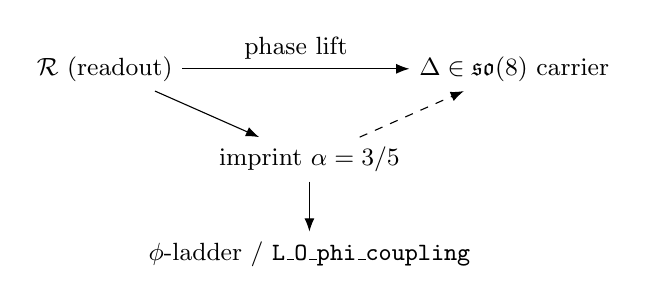
\begin{tikzpicture}[font=\small,>=Latex]
\node (R) at (0,0) {$\mathcal{R}$ (readout)};
\node (D) at (5.2,0) {$\Delta\in\mathfrak{so}(8)$ carrier};
\node (a) at (2.6,-1.15) {imprint \(\alpha=3/5\)};
\node (phi) at (2.6,-2.35) {\(\phi\)-ladder / \texttt{L\_O\_phi\_coupling}};
\draw[->] (R) -- node[above]{phase lift} (D);
\draw[->] (R) -- (a);
\draw[->,dashed] (a) -- (D);
\draw[->] (a) -- (phi);
\end{tikzpicture}
\caption{Design bridge (schematic): the readout pipeline fixes \(\Delta\) in the skew-adjoint octonionic carrier while the curvature imprint \(\alpha\) feeds the auxiliary-field ladder and the action's \(\phi\)-coupling. A fully functorial arrow \(\mathcal{R}\rightsquigarrow A\) is not yet formalized (see \hyperref[lean:scaffold-bridge]{manifold-Lagrangian scaffold and lattice/continuum coincidence}); Subsection~\ref{subsec:minimal-seed} gives an explicit Stokes-compatible seed on the minimal \(\mathrm{Fin}\,4\) cycle.}
\label{fig:bridge}
\end{figure}

\subsection{Functoriality gap}

A patch-internal morphism \(\mathcal{R}\rightsquigarrow A\) with bookkeeping estimates as the patch class is enlarged (more shells, larger cycles, wider auxiliary ladders) is parked inside the \hyperref[lean:scaffold-bridge]{manifold-Lagrangian scaffold and lattice/continuum coincidence interface}. Subsection~\ref{subsec:minimal-seed} gives the reference-plaquette seed already certified as the \hyperref[lean:readout-seed]{minimal readout-to-gauge seed on the \(\mathrm{Fin}\,4\) cycle}; functorial extension to larger discrete patches, and any continuum-coordinate rewrites used only for cross-citation, are Tier~III \emph{calculation-approximation} translation tasks (Sect.~\ref{sec:outlook}). They are \emph{not} an HQIV open problem: the discrete EL identity, the cyclic flux sum, and the two-sided Wilson bound are the load-bearing statements at the patch layer, and any continuum-notation readout sits on top of them as an optional comparison artefact---never as an underlying ontology (\S``Patch QFT and discrete numerics'' above).

\subsection{Minimal seed map \texorpdfstring{$\mathcal{R}\rightsquigarrow A$}{R to A} on the reference \texorpdfstring{$\mathrm{Fin}\,4$}{Fin4} cycle}
\label{subsec:minimal-seed}

This subsection packages a single, fully explicit assignment from the normalized readout and auxiliary ladder to edge fluxes on the smallest nontrivial spacetime cycle, compatible with Lemma~\ref{lem:stokes} and with the abelian holonomy lemmas of Sect.~\ref{sec:holonomy}. The same assignment is the \hyperref[lean:readout-seed]{minimal readout-to-gauge seed on the \(\mathrm{Fin}\,4\) cycle}; it is the natural first discrete closure of Figure~\ref{fig:bridge} on one plaquette, fully internal to the discrete patch layer (no continuum limit is invoked or required).

\paragraph{Setup.}
Fix the calibration shell \(m=m_{\mathrm{ref}}\) (definitionally tied to the QCD-onset ladder; numerically \(4\) in the current repository constants). Under positivity of the curvature integral at \(m_{\mathrm{ref}}\), the partial curvature ratio satisfies \(\Omega_k(m_{\mathrm{ref}};m_{\mathrm{ref}})=1\)---the discrete normalization pin for the \(\Omega\) layer in \cite{hqiv-so8-paper}. Write \(\mathcal{R}(n)\) for the normalized cumulative readout at shell \(n\), and \(\phi(n)=2(n+1)\) for the auxiliary scalar from the \hyperref[lean:phi-ladder]{auxiliary field ladder}. Define the per-shell readout increment
\[
\delta_{\mathcal{R}}(n):=\mathcal{R}(n+1)-\mathcal{R}(n),
\]
and the imprint-weighted phase increment
\begin{equation}
\label{eq:omega-n}
\omega(n):=\alpha\,\log\bigl(\phi(n)+1\bigr)\,\delta_{\mathcal{R}}(n),
\end{equation}
with \(\alpha=3/5\). The phase-lift generator \(\Delta\in\mathfrak{so}(8)\) is fixed in the \((e_1,e_7)\) plane in the HQVM conventions of \cite{hqiv-so8-paper}; let \(\theta\) denote the corresponding polar angle in that plane and set
\[
v^1:=\cos\theta,\qquad v^7:=\sin\theta,\qquad v^a:=0\ \ (a\notin\{1,7\}),
\]
so \(v\in\mathbb{R}^8\) is a unit vector in the \(\Delta\)-direction.

\paragraph{Stokes-compatible flux on the \(\mathrm{Fin}\,4\) cycle.}
For a \emph{fixed} shell label \(n\), assign internal components on directed edges \(i\to i+1\) of the cyclic \(\mathrm{Fin}\,4\) graph by
\begin{equation}
\label{eq:seed-F}
F^1_{i,i+1}(n)=\omega(n)\,s_i\,\cos\theta,\qquad
F^7_{i,i+1}(n)=\omega(n)\,s_i\,\sin\theta,\qquad
F^a_{i,i+1}(n)=0\ \ (a\notin\{1,7\}),
\end{equation}
where \((s_0,s_1,s_2,s_3)=(+1,+1,-1,-1)\). Then \(\sum_{i\in \mathrm{Fin}\,4} F^a_{i,i+1}(n)=0\) for every \(a\) and every \(n\), so Lemma~\ref{lem:stokes} holds \emph{by construction}. Recover potentials on vertices by fixing \(A^a_0(n)=0\) and defining
\[
A^a_{i+1}(n):=A^a_i(n)+F^a_{i,i+1}(n)\qquad (i=0,1,2,3),
\]
with indices interpreted cyclically so that \(A^a_4(n)=A^a_0(n)\); this is the standard pure-gauge freedom on a loop: only the edge data enter the \hyperref[lean:F-from-A]{discrete field strength}, the \hyperref[lean:LO-kinetic]{kinetic density}, and the holonomy glue.

\paragraph{Verification (three checks).}
\begin{enumerate}
\item \textbf{Cyclic flux (Lemma~\ref{lem:stokes}).} The choice~\eqref{eq:seed-F} forces \(\sum_i F^a_{i,i+1}(n)=0\) by the alternating signs; equivalently, the vertex potential closes after four steps. No octonion multiplication is used---only \(\mathbb{R}\)-addition, matching the discrete Stokes proof style.
\item \textbf{Abelian holonomy (Lemma~\ref{lem:hol-one}).} Cyclic transport is built from \(\mathbb{R}\)-translation applied to the edge variables \(F^a_{i,i+1}\); Lemma~\ref{lem:hol-one} gives the identity holonomy whenever the cyclic sum vanishes. Thus the seed is automatically compatible with the proved \(\mathbb{R}\)-translation picture. An \emph{interpretive} upgrade identifies \(\omega(n)\,v\) with an infinitesimal rotation in the \(\Delta\)-plane inside \(\mathfrak{so}(8)\); the exponential \(\exp(\cdot\,\Delta)\) language belongs to that matrix sector and is not literal \(\mathbb{R}\)-translation composition until a non-abelian transport layer is wired (\hyperref[lean:non-abelian-pointer]{non-abelian holonomy pointer}).
\item \textbf{Reference normalization.} At the calibration shell \(m_{\mathrm{ref}}\), \(\omega(n)\) vanishes whenever \(\delta_{\mathcal{R}}(n)=0\) at that shell (e.g.\ a bookkeeping pivot for the readout increment); then~\eqref{eq:seed-F} collapses to \(F=0\) and, with \(A(\cdot,n)\equiv 0\) at the base vertex, to the flat cycle used in Example~\ref{ex:simultaneous}. More generally, \(\omega(n)\) couples the curvature channel through \(\delta_{\mathcal{R}}\) and the auxiliary factor \(\log(\phi(n)+1)\) that already appears in \(\mathcal{L}_\phi\) (Sect.~\ref{sec:discrete}); the closed form \(\phi(n)=2(n+1)\) is independent of the Friedmann \(\phi_{\mathrm{val}}\) normalization in the action cell unless explicitly identified.
\end{enumerate}

\paragraph{Sign-pattern equivalence under the global \(\mathrm{SO}(8)\) action.}
The choice \((s_0,s_1,s_2,s_3)=(+1,+1,-1,-1)\) is one of several alternating sign patterns on \(\mathrm{Fin}\,4\) compatible with the cyclic-flux constraint of Lemma~\ref{lem:stokes}. Within the polynomial gauge ansatz of Tier~I, the equivalence class of admissible patterns is described by the following observation, which is the right ``Tier-I uniqueness up to global symmetry'' statement.

\begin{proposition}[Seed equivalence on the minimal cycle]
\label{prop:seed-equivalence}
Let \(s,s'\in\{\pm 1\}^{\mathrm{Fin}\,4}\) satisfy \(\sum_i s_i=\sum_i s'_i=0\) (the cyclic-flux closure condition). Then the seed gauge potentials \(A_{s,v},A_{s',v}\) constructed from~\eqref{eq:seed-F} with sign vectors \(s,s'\) and the same unit vector \(v\in\mathbb{R}^8\) supported in the \((e_1,e_7)\) plane are related by an \(\mathrm{Fin}\,4\)-cyclic relabelling of vertices composed with a sign-flip on the orientation of the \(\Delta\)-plane, and yield isomorphic data for the \hyperref[lean:F-from-A]{discrete field strength}, the \hyperref[lean:LO-kinetic]{kinetic density}, and the cyclic holonomy. Equivalently, in the \emph{interpretive} \(\mathfrak{so}(8)\) reading of the seed, all such choices lie on a single global \(\mathrm{SO}(8)\) orbit of the canonical seed \((+1,+1,-1,-1)\).
\end{proposition}

\begin{proof}[Sketch]
There are exactly six binary vectors \(s\in\{\pm 1\}^4\) with \(\sum_i s_i=0\) (choose two positions for \(+1\)). The four ``alternating-block'' patterns \((+,+,-,-),(-,+,+,-),(-,-,+,+),(+,-,-,+)\) are cyclic shifts of one another and produce the same edge data up to a relabelling of \(\mathrm{Fin}\,4\); the remaining two ``checkerboard'' patterns \((+,-,+,-)\) and \((-,+,-,+)\) flip the orientation of the cycle and are absorbed into a sign change of \(v\) (equivalently, of the polar angle \(\theta\to\theta+\pi\) in the \((e_1,e_7)\) plane). The kinetic density \(\mathcal{L}_{\mathrm{kin}}\) is invariant under both moves because it is a sum of squares of edge fluxes, and the cyclic holonomy is invariant because the cyclic flux sum vanishes for every choice. The interpretive embedding \(\omega(n)\,v\hookrightarrow\mathfrak{so}(8)\) sends both moves to global \(\mathrm{SO}(8)\) rotations preserving the \((e_1,e_7)\) plane.
\end{proof}

In particular, the canonical seed used in Lean is one representative of a single \(\mathrm{SO}(8)\)-orbit, not an extra choice over and above the predecessor papers' identification of the \((e_1,e_7)\) plane: any other admissible alternating pattern produces a globally rotated copy of the same theory.

\paragraph{Status and scope.}
The \hyperref[lean:readout-seed]{minimal readout-to-gauge seed module} certifies the alternating-edge pattern of~\eqref{eq:seed-F}, the corresponding gauge potential, and the readout-linked phase \(\omega(n)\); the cyclic flux sum and trivial discrete holonomy are specialized to this seed; flat degeneration is recorded when the curvature-ratio increment vanishes shell-to-shell. What remains outside Lean is promoting shell-indexed potentials \(A(\cdot,n)\) to a global variational field in the action layer, proving functoriality and mesh-refinement estimates, and upgrading the abelian translation transport to matrix \(\exp(\cdot\,\Delta)\) data---the Tier~III programme in Sect.~\ref{sec:outlook}.

\section{Tiered uniqueness thesis}
\label{sec:tiers}

\subsection{Tier I: EL slot rigidity (formal layer)}

In continuum polynomial abelian gauge theory, \(\mathcal{L}\sim -\tfrac14 F_{\mu\nu}F^{\mu\nu}+J_\mu A^\mu\) yields \(\partial_\mu F^{\mu\nu}=4\pi J^\nu\) up to gauge-fixing nuances. The discrete HQIV choice replaces \(\partial_\mu\) by the finite-difference operator whose quadratic form is exactly~\eqref{eq:Lkin-expanded}; Theorem~\ref{thm:EL} is therefore the \emph{same} uniqueness of functional derivative up to the declared \(J\) and \(\phi\) slots, proved by unfolding the relevant definitions (\hyperref[lean:EL-divergence]{discrete EL identity}).

\paragraph{Finite-difference dictionary.}
If one thinks of \(\mu\in\mathrm{Fin}\,4\) as labeling vertices of a periodic one-cell graph, then \(F^a{}_{\mu\nu}\) is the oriented edge jump from \(\mu\) to \(\nu\). The EL expression \(\sum_\mu F^a{}_{\mu\nu}\) is the net flux out of vertex \(\nu\) after summing over all partners \(\mu\): the same combinatorial object that becomes \(\partial_\mu F^{\mu\nu}\) after mesh refinement under uniform bounds on \(A\). Thus Tier~I is not an \emph{ad hoc} discrete trick; it is the standard Maxwell EL with honest finite differences on the HQIV index set.

\paragraph{What is \emph{not} determined at Tier~I.}
Adding total ``discrete divergences'' that vanish identically on every \(A\) would change \(\mathcal{L}\) by a null Lagrangian without changing EL; the HQIV file fixes a definite representative (the normalized \(F^2\) sum~\eqref{eq:Lkin-expanded}). Uniqueness claims at Tier~I are therefore uniqueness of the \emph{chosen} representative's EL slot, not uniqueness of all possible discrete prelimits of the same continuum theory.

\paragraph{Side-by-side dictionary.}
Table~\ref{tab:dictionary} positions the HQIV discrete EL alongside the two natural neighbours: the continuum Maxwell action and the Wilson plaquette action of standard lattice gauge theory. The point is not that the three are the same theory, but that the HQIV variational layer cleanly inherits the EL/source structure from continuum Maxwell and the cyclic-edge data from Wilson, while keeping the \emph{patch} ontology that neither continuum Maxwell nor Wilson lattice gauge theory adopts.

\begin{table}[ht]
\caption{HQIV discrete EL vs.\ continuum Maxwell vs.\ Wilson plaquette action: roles of the basic objects and ontological status.}
\label{tab:dictionary}
\centering
\footnotesize
\begin{tabular}{@{}p{3.0cm}p{3.4cm}p{3.4cm}p{3.4cm}@{}}
\hline
Object & HQIV (this paper) & Continuum Maxwell & Wilson lattice \cite{wilson1974,creutz1983}\\
\hline
Carrier & \(A^a{}_\mu\) on \(\mathrm{Fin}\,8\times\mathrm{Fin}\,4\) & \(A_\mu\in\Omega^1(M)\) on smooth \(M\) & \(U_\ell\in G\) on lattice links \(\ell\)\\
Field strength & \(F^a{}_{\mu\nu}=A^a{}_\nu-A^a{}_\mu\) (algebraic) & \(F_{\mu\nu}=\partial_\mu A_\nu-\partial_\nu A_\mu\) (differential) & \(U_p=\prod_{\ell\in\partial p}U_\ell\) (plaquette) \\
Action & \(-\tfrac{1}{4}\sum F^2/2 + 4\pi J\!\cdot\!A + \mathcal{L}_\phi\) & \(\int(-\tfrac{1}{4}F_{\mu\nu}F^{\mu\nu}+J_\mu A^\mu)\,d^4x\) & \(\beta\sum_p\mathrm{Re}\,\mathrm{tr}(1-U_p)\) \\
EL / variation & \(\sum_\mu F^a{}_{\mu\nu}=4\pi J^a{}_\nu\) (\hyperref[lean:EL-divergence]{Theorem~\ref{thm:EL}}) & \(\partial_\mu F^{\mu\nu}=4\pi J^\nu\) & \(\partial S/\partial U_\ell=0\) (saddle point in \(U\)) \\
Holonomy & Cyclic Stokes \(\sum_i F^a{}_{i,i+1}=0\) and trivial cyclic plaquette holonomy in \(\mathbb{R}\) & Stokes' theorem \(\oint A=\int F\) & Plaquette holonomy \(U_p\); confinement test on \(\langle\mathrm{tr}\,U_p\rangle\) \\
Coercive bound & Two-sided \(-\tfrac12\Sigma\le\mathcal{L}_{\mathrm{kin}}\le-\tfrac14\Sigma\) on cyclic Wilson squares (Lemma~\ref{lem:wilson-bounds}) & Energy \(\tfrac12(E^2+B^2)\ge 0\) & Strong-coupling expansion in \(\beta\); area law for Wilson loops \\
Ontology & \emph{Patch theory}: discrete is fundamental & Continuum is fundamental; lattice is approximation & Discrete \emph{regulator} for continuum QFT (\(a\to 0\) UV limit) \\
\hline
\end{tabular}
\end{table}

\subsection{Tier II: division algebra and eight channels (classical layer)}

Hurwitz's theorem classifies finite-dimensional normed division \(\mathbb{R}\)-algebras as \(\mathbb{R},\mathbb{C},\mathbb{H},\mathbb{O}\) \cite{baez2002,springer2000}. Baez emphasizes the ``normed division algebra ladder'' stopping at \(\mathbb{O}\); Springer--Veldkamp supply the standard structure theory (alternative algebras, norm forms, \(\mathrm{Aut}(\mathbb{O})=G_2\)). Only \(\mathbb{O}\) has real dimension \(8\), matching the \(\mathrm{Fin}\,8\) carrier and the \(\mathrm{Spin}(8)\) triality story reviewed in \cite{hqiv-3d-growth-paper}. Once the HQVM matrices and \(\Delta\) are fixed, the machine-checked closure \(G_2\cup\{\Delta\}\Rightarrow\mathfrak{so}(8)\) of \cite{hqiv-so8-paper} pins an exceptional \(28\)-dimensional bracket envelope on that carrier. Tier~II uniqueness is therefore \emph{algebraic compatibility}: the octonions are the unique normed division algebra of the dimension required for this particular closure package.

\paragraph{Triality as a selection rule (informal).}
Among division algebras, only the \(8\)-dimensional case carries outer automorphisms of \(\mathrm{Spin}(8)\) large enough to coordinate vector, spinor, and conjugate-spinor roles in the way the HQIV narrative packages internal quantum numbers. The present paper does not reprove triality; it records that the Lean closure certificate is \emph{specialized} to the octonionic \(8\times 8\) seed, so any alternate division-algebra carrier would require a fresh closure script of comparable strength.

\subsection{Tier III: program (patch-internal interoperability layer)}
\label{subsec:tierIII}

\paragraph{Scope (mandatory clarification).}
Tier III is \emph{not} a programme to recover or approach a continuum limit. Per the patch-theory reader contract, the discrete patch layer is the ontology, the observable universe \emph{is} the whole universe in HQIV, and several Tier-I results would be erased rather than refined by an ultraviolet/mesh continuum limit (e.g.\ the rational shell coefficients, the integer cycle indices that carry the holonomy bound, and the discrete index that the predictive ladder runs on). Whatever Tier III contributes, it must respect that ontology: the discrete patch layer remains primary, and continuum notation is admitted only as a calculation-approximation rewrite for cross-citation with literature that happens to use that language.

We therefore isolate three explicit open sub-problems, all formulated entirely inside the patch ontology:
\begin{enumerate}
\item \textbf{Patch-to-literature translation rewrites.} Construct controlled \emph{translations} from \(\mathcal{R}\) (and shell ledgers) to the connection/curvature notation used in the standard literature, treated as calculation-approximation coordinates---\emph{not} as definitions and \emph{not} as an underlying theory of which the patch layer is a discretization. The role of these rewrites is interoperability and cross-citation; the bookkeeping must record where the rewrite is injective, where information is lost, and which discrete indices have no continuum image.
\item \textbf{Paired patch stationarity.} Promote \(\mathcal{S}_{\mathrm{tot}}\) to a stationary functional over an enlarged \emph{discrete} patch class (more shells, larger cycles, wider auxiliary ladders) whose discrete EL system carries a paired gauge/gravity constraint. The target is a discrete analogue of paired Einstein/\(G_2\) stationarity packaged as a patch theorem; no continuum limit is taken.
\item \textbf{Associator-weighted discrete measure.} Encode the octonionic associator \((x,y,z)\) in a weighting on the discrete patch path-counting measure (still finite/discrete) so that quaternionic and sedenionic truncations fail structurally on patch data. The output is a discrete amplitude, not a continuum path integral.
\end{enumerate}

The three sub-problems are connected by the same \((\alpha,\phi)\) ledger: each adds patch-internal structure on top of the certified Tier-I core without changing what the foundational objects \emph{are}.

\section{Quantum scaffold and forward compatibility}
\label{sec:quantum}

The HQIV Hamiltonian template is realized as a Lean predicate by the \hyperref[lean:schrodinger]{Schr\"odinger scaffold}: the extended-action EL is definitionally the Schr\"odinger predicate. Placeholder Laplacians remain; when Tier~III supplies the associator-weighted discrete measure of \S\ref{subsec:tierIII}, this scaffold is the natural place to assert summability and variational well-posedness on patch data compatible with that weighting, including discrete BRST or BV upgrades if the associator enters as a constraint closing ghost sectors.

\section{Outlook and roadmap for Tier III}
\label{sec:outlook}

\subsection{Minimal additional Lean scaffolds}

The items below are patch-internal extensions in the sense of \S\ref{subsec:tierIII}: each adds discrete structure or explicit translation rewrites on top of the certified Tier-I core; none promotes a continuum limit to definitional status.

\begin{itemize}
\item Promote the \hyperref[lean:scaffold-bridge]{manifold-Lagrangian scaffold and lattice/continuum coincidence} interface from a hypothesis structure to a theorem template comparing patch sums against the standard-literature integrals they translate to (calculation-approximation only; the Lean module retains the name \texttt{LatticeContinuumActionCoincidence} as a literal identifier).
\item Controlled \emph{patch} bridge lemmas \(\mathcal{R}\rightsquigarrow A\) (or \(\Delta\rightsquigarrow A\)) on enlarged discrete patches, with explicit bookkeeping as cycle/shell counts grow.
\item Discrete-measure weighting slot for the octonionic associator, and quaternionic/sedenionic obstruction lemmas stated as \texttt{false} targets under the same ansatz.
\item Wire the gradient-component slot of the modified-Maxwell module fully through both the discrete EL and the emergent inhomogeneous Maxwell formulations on charts to close the action / modified-Maxwell loop (Remark~\ref{rem:modified-maxwell}); this is a literature-translation rewrite, not a redefinition of HQIV in continuum terms.
\end{itemize}

\subsection{Milestone ordering (suggested)}

\begin{enumerate}
\item Close the action / modified-Maxwell gradient-slot identification on charts (translation rewrite, patch-internal).
\item Promote the lattice/continuum coincidence interface to an explicit-rate theorem comparing patch sums to literature integrals.
\item Build a functor \(\mathcal{R}\rightsquigarrow A\) on a restricted class of patch configurations (partial maps first, bookkeeping second).
\item Add non-abelian holonomy lemmas mirroring the \hyperref[lean:wilson-bounds]{two-sided Wilson bound} for matrix transports (\hyperref[lean:non-abelian-pointer]{non-abelian holonomy pointer}).
\item Promote the \hyperref[lean:weakHiggs-scaffold]{weak/Higgs Tier-III scaffold} from reduction-level theorems to a full EL package for weak channels and scalar sector.
\item Encode associator weights in a discrete patch measure; prove quaternionic obstruction lemmas.
\item Revisit the \hyperref[lean:schrodinger]{Schr\"odinger scaffold} once a discrete measure is fixed, upgrading placeholders to certified patch operators.
\end{enumerate}

\subsection{Dependency sketch (text)}

\[
\begin{aligned}
&\text{Growth }(\rho,K,\Omega,\mathcal{R}) &&\longrightarrow &&\alpha,\ \phi\text{-ladder} \\
&\quad\Downarrow && &&\quad\Downarrow \\
&\Delta,\ G_2\text{ seed} &&\longrightarrow &&\mathfrak{so}(8)\text{ closure} \quad \text{\cite{hqiv-so8-paper}}\\
&\quad && &&\quad\Downarrow \\
& && &&\text{Action } \mathcal{S}_{\mathrm{tot}}\quad\text{(this paper, \S\ref{sec:discrete}--\ref{sec:grav})}\\
&\quad && &&\quad\Downarrow \\
& && &&\text{Holonomy/Wilson packaging (\S\ref{sec:holonomy})}\\
&\quad && &&\quad\Downarrow \\
& && &&\text{Tier III (patch-internal): translation rewrites, paired stationarity,}\\
& && &&\text{associator-weighted discrete measure (future work).}
\end{aligned}
\]

\subsection{Thermodynamic root and lattice gauge vocabulary}

Jacobson's thermodynamic state relation for spacetime \cite{jacobson1995} is the standard conceptual ancestor of ``Einstein equation of state'' arguments; Brodie's horizon package \cite{brodie2026} is the imported normalization route for \(\alpha=3/5\) in the HQIV growth papers and feeds the same imprint into \(\mathcal{L}_\phi\) and \(G_{\mathrm{eff}}\) here. Separately, Wilson's lattice link variables \cite{wilson1974} and the textbook discrete gauge theory framework \cite{creutz1983} supply the vocabulary for reading Lemma~\ref{lem:wilson-bounds} as a small-flux plaquette inequality: the HQIV glue lemmas are not a new lattice gauge theory, but they position the O--Maxwell kinetic where Wilson-type estimates can be imported when Tier~III tightens scalings.

\appendix

\section{Lean module index}
\label{app:lean-index}

The Lean development lives in the public slimmed mirror \url{https://github.com/HQIV/hqiv-lean} \cite{hqiv-lean}. All cited theorems are sorry-free at the time of writing. Each entry below carries a reader-friendly anchor (used by hyperlinks in the body), a one-line description, and clickable links to the Lean module and identifiers.

\begingroup
\sloppy
\setlength{\emergencystretch}{5em}
\begin{description}[leftmargin=*]
  \item[\phantomsection\label{lean:F-from-A}\textbf{Discrete field strength.}]
    The lattice analogue of \(F_{\mu\nu}=\partial_\mu A_\nu-\partial_\nu A_\mu\) on the \(\mathrm{Fin}\,4\) cycle: \(F^a{}_{\mu\nu}(A)=A^a{}_\nu-A^a{}_\mu\). Lean: \leanid{F_from_A} in \leanfile{Hqiv/Physics/Action.lean}.

  \item[\phantomsection\label{lean:LO-kinetic}\textbf{Kinetic, source, and \texorpdfstring{\(\phi\)}{phi}-coupling densities.}]
    The three additive pieces of the O--Maxwell Lagrangian: a normalized \(F^2\) sum, a \(J\!\cdot\!A\) source coupling, and a \(\phi\)-coupling carrying the imprint \(\alpha=3/5\) on channel \(a=0\). Lean: \leanid{L_O_kinetic}, \leanid{L_O_source_general}, \leanid{L_O_phi_coupling} in \leanfile{Hqiv/Physics/Action.lean}; the gradient slot \leanid{grad_phi} is a placeholder in the same file (continuum gradients live in \leanfile{Hqiv/Physics/ContinuumOmaxwellClosure.lean} as \leanid{coordsGradientComponents}).

  \item[\phantomsection\label{lean:LO-Maxwell}\textbf{Full O--Maxwell density and action cell.}]
    The total density \(\mathcal{L}_O=\mathcal{L}_{\mathrm{kin}}+4\pi\mathcal{L}_{\mathrm{src}}+\mathcal{L}_\phi\) and the corresponding numerical action cell. Lean: \leanid{L_O_Maxwell_general} and \leanid{action_O_Maxwell_general} in \leanfile{Hqiv/Physics/Action.lean}.

  \item[\phantomsection\label{lean:EL-divergence}\textbf{Discrete EL identity.}]
    The Euler--Lagrange covector at \((a,\nu)\) equals \(\sum_\mu F^a{}_{\mu\nu}-4\pi J^a{}_\nu\) (with the \(\phi\)-correction on channel \(a=0\)); this is the discrete analogue of \(\partial_\mu F^{\mu\nu}=4\pi J^\nu\). Lean: \leanid{EL_O_general}, \leanid{action_O_Maxwell_EL_eq_emergent_general} (and \leanid{action_O_Maxwell_EL_eq_emergent} for the canonical \leanid{J_O} current), and \leanid{EL_O_general_eq_F_divergence_sub_sources}, all in \leanfile{Hqiv/Physics/Action.lean}.

  \item[\phantomsection\label{lean:add-J}\textbf{Source superposition correction.}]
    The bookkeeping correction enforcing ``no double counting'' of the kinetic, \(\phi\), and gravity pieces when concatenating two sources \(J_1+J_2\) into one variational cell. Lean: \leanid{action_O_Maxwell_general_add_J} and \leanid{action_total_general_add_J} in \leanfile{Hqiv/Physics/Action.lean}.

  \item[\phantomsection\label{lean:S-grav}\textbf{Gravitational constraint as Friedmann.}]
    The HQVM gravity action \(\mathcal{S}_{\mathrm{grav}}\) vanishes iff the HQVM Friedmann identity holds; for \(\phi\ge 0\) the constraint reads \((13/5)\phi^2 = 8\pi\,\phi^{\alpha}(\rho_m+\rho_r)\). Lean: \leanid{S_HQVM_grav}, \leanid{S_HQVM_grav_zero_iff_Friedmann}, and \leanid{O_Maxwell_compatible_with_HQVM_GR_homogeneous} in \leanfile{Hqiv/Physics/Action.lean} and \leanfile{Hqiv/Physics/GRFromMaxwell.lean}; the prefactor identity \((3-\gamma_{\mathrm{HQIV}})=13/5\) is \leanid{three_minus_gamma_eq} in \leanfile{Hqiv/Geometry/HQVMetric.lean}, and \leanid{G_eff_eq} ((\(G_{\mathrm{eff}}(\phi)=\phi^{\alpha}\)), with \leanid{G0_eq} as natural-unit normalization) lives in \leanfile{Hqiv/Physics/GRFromMaxwell.lean}.

  \item[\phantomsection\label{lean:total-action}\textbf{Total action and joint EL/Friedmann packaging.}]
    The total cell \(\mathcal{S}_{\mathrm{tot}}=\mathcal{S}_O+\mathcal{S}_{\mathrm{grav}}\) and the joint statement that gravity arises as a constraint while the gauge sector's EL is the discrete equation of motion at the chosen potential. Lean: \leanid{action_total_general} and \leanid{equations_from_action} in \leanfile{Hqiv/Physics/Action.lean}.

  \item[\phantomsection\label{lean:cyclic-flux}\textbf{Discrete Stokes (cyclic flux sum).}]
    For every channel \(a\) and every potential \(A\), \(\sum_{i\in\mathrm{Fin}\,4} F^a{}_{i,i+1}(A)=0\); the discrete face of Stokes' theorem on the minimal spacetime cycle. Lean: \leanid{sum_F_cyclicIndex_eq_zero} in \leanfile{Hqiv/Physics/ActionHolonomyGlue.lean}.

  \item[\phantomsection\label{lean:trivial-holonomy}\textbf{Trivial cyclic plaquette holonomy.}]
    Cyclic transport built from \(\mathbb{R}\)-translation operators on the edges \(F^a{}_{i,i+1}\) returns the identity. Lean: \leanid{discreteSquareHolonomy_F_cyclic_eq_one} (with edge transports \leanid{linearEnd}) in \leanfile{Hqiv/Physics/ActionHolonomyGlue.lean}.

  \item[\phantomsection\label{lean:wilson-bounds}\textbf{Two-sided Wilson bound on the kinetic aggregate.}]
    \(-\tfrac12\sum (U^a_i x-x)^2 \le \mathcal{L}_{\mathrm{kin}}(A) \le -\tfrac14\sum (U^a_i x-x)^2\) for every \(x\in\mathbb{R}\), where \(U^a_i\) are the cyclic edge translations. Lean: \leanid{L_O_kinetic_le_neg_quarter_sum_cyclic_wilson_sq}, \leanid{L_O_kinetic_ge_neg_half_sum_cyclic_wilson_sq}, and \leanid{L_O_kinetic_two_sided_cyclic_wilson_sq} in \leanfile{Hqiv/Physics/ActionHolonomyGlue.lean}.

  \item[\phantomsection\label{lean:emergent-maxwell}\textbf{Emergent inhomogeneous Maxwell slot.}]
    The companion file packaging the same \(-4\pi J_{\mathrm{src}}\) source slot and \(\alpha\)-weighted \(\phi\)-gradient correction; the maintained design contract is source-slot alignment between EL and the emergent inhomogeneous equation. Lean: \leanid{emergentMaxwellInhomogeneous_O_general} and \leanid{emergentMaxwellInhomogeneous_O_coordsField} in \leanfile{Hqiv/Physics/ModifiedMaxwell.lean}.

  \item[\phantomsection\label{lean:lapse-bridge}\textbf{Lapse dragging: shared \texorpdfstring{$\phi$}{phi} and \texorpdfstring{$\alpha$}{alpha} across O--Maxwell and GR.}]
    The HQVM lapse \(N=1+\Phi+\phi t/c\), with the same auxiliary scalar \(\phi\) entering the O--Maxwell \(\phi\)-coupling and the homogeneous GR branch. Lean: \leanid{HQVM_lapse} in \leanfile{Hqiv/Geometry/HQVMetric.lean} and \leanid{same_phi_in_O_Maxwell_and_HQVM}, \leanid{same_alpha_in_O_Maxwell_and_HQVM} in \leanfile{Hqiv/Physics/GRFromMaxwell.lean}.

  \item[\phantomsection\label{lean:phi-ladder}\textbf{Auxiliary field ladder.}]
    The temperature-tied auxiliary scalar \(\phi(m)=2(m+1)\): \leanid{phi_of_shell} divided by \leanid{T} at shell index \(m\), with \leanid{phiTemperatureCoeff} the proved constant \(2\) (\leanid{phiTemperatureCoeff_eq_two}) and the closed form \leanid{phi_of_shell_closed_form}. The shell readout rewrite \(\phi(m)/2=m+1\) is \leanid{shell_shape_in_terms_of_phi}, all in \leanfile{Hqiv/Geometry/AuxiliaryField.lean}.

  \item[\phantomsection\label{lean:imprint-alpha}\textbf{Curvature imprint \texorpdfstring{$\alpha=3/5$}{alpha = 3/5}.}]
    The forced rational identity \(\alpha=3/5\) on the discrete light-cone, together with the shell shape and reference normalization. Lean: \leanid{alpha_eq_3_5}, \leanid{shell_shape}, \leanid{omega_k_partial_at_reference}, and \leanid{referenceM} in \leanfile{Hqiv/Geometry/OctonionicLightCone.lean}.

  \item[\phantomsection\label{lean:readout-seed}\textbf{Minimal readout-to-gauge seed on the \texorpdfstring{$\mathrm{Fin}\,4$}{Fin 4} cycle.}]
    The explicit Stokes-compatible vertex/edge profile linking the normalized cumulative readout \(\mathcal{R}\) and auxiliary ladder \(\phi(n)\) to a discrete gauge potential on the minimal spacetime cycle, with proofs that the cyclic flux sum vanishes and the cyclic holonomy is trivial. Lean: \leanid{seedAProfileAux}, \leanid{seedPotentialMinimalCycle}, \leanid{imprintWeightedReadoutPhase}, \leanid{seedPotentialMinimalCycle_cyclic_sum_F}, \leanid{seedPotentialMinimalCycle_discrete_holonomy_one}, and \leanid{seedPotentialMinimalCycle_of_imprint_increment_zero} in \leanfile{Hqiv/Physics/ReadoutGaugeSeed.lean}.

  \item[\phantomsection\label{lean:scaffold-bridge}\textbf{Manifold-Lagrangian scaffold and lattice/continuum coincidence.}]
    Optional manifold-integration wrappers carrying the variational layer to chart pullbacks, and the hypothesis structure used to compare a discrete sum to a continuum integral. Lean: \leanid{LagrangianDensity} in \leanfile{Hqiv/Geometry/ManifoldLagrangianScaffold.lean} and \leanid{LatticeContinuumActionCoincidence} (currently a hypothesis interface; see Sect.~\ref{sec:outlook}).

  \item[\phantomsection\label{lean:weakHiggs-scaffold}\textbf{Weak/Higgs Tier-III scaffold and reductions.}]
    A typed extension surface carrying a weak field strength, weak kinetic density, octonion-carrier scalar, quartic Higgs potential, and lock-in vev proxy, together with theorem-level reductions back to the proved abelian action when extension slots are switched off. Lean: \leanid{WeakIdx}, \leanid{WeakPotential}, \leanid{WeakCommTerm}, \leanid{weakF}, \leanid{L_weak_kinetic}, \leanid{scalarNormSq}, \leanid{higgsPotential}, \leanid{lockinVev}, \leanid{weakF_reduces_to_abelian}, \leanid{weakF_diag_eq_zero_of_abelian}, \leanid{lockinVev_sq_eq_eta_paper}, \leanid{lockinVev_eq_sqrt_eta_paper}, \leanid{omega_k_lockin_calibration}, \leanid{action_O_weak_higgs_reduces_to_action_O_Maxwell}, \leanid{action_O_weak_higgs_reduces_exactly_to_action_O_Maxwell}, and \leanid{weakHiggs_triality_tilt_average_eq_one} in \leanfile{Hqiv/Physics/WeakHiggsFromOMaxwellScaffold.lean}.

  \item[\phantomsection\label{lean:schrodinger}\textbf{Schr\"odinger scaffold from the extended-action EL.}]
    The HQIV Hamiltonian template realized as a Lean predicate; the extended-action EL is definitionally the Schr\"odinger scaffold for square-integrable upgrades in Tier~III. Lean: \leanid{eulerLagrange_eq_Schrodinger} and \leanid{actionExtensionYieldsSchrodinger} in \leanfile{Hqiv/QuantumMechanics/Schrodinger.lean}.

  \item[\phantomsection\label{lean:non-abelian-pointer}\textbf{Non-abelian holonomy pointer.}]
    Matrix-valued transports inside \texttt{Function.End} on the same combinatorial cycle, carrying the natural non-abelian upgrade of the abelian Wilson packaging in \hyperref[lean:wilson-bounds]{the kinetic--Wilson bound}. Lean: \leanfile{Hqiv/Physics/DiscretePlaquetteHolonomy.lean}.
\end{description}
\endgroup

\subsection{Lake build targets}
\label{subsec:lake-targets}

The HQIV-LEAN checkout splits heavy certification across named \texttt{lake build} targets so that the variational cone is not conflated with optional matrix tables.
\begingroup
\sloppy
\setlength{\emergencystretch}{4em}
\begin{itemize}
  \item \textbf{Manuscript / appendix cone:} \texttt{lake build HQIVPaperClaims} elaborates the action / EL / holonomy chain together with the symbolic \(\mathfrak{so}(8)\) interface, without the floating-point Lie-bracket cell cone.
  \item \textbf{Default library cone:} \texttt{lake build HQIVLEAN} is the main import surface used by narrative modules such as the action and holonomy theorems above.
  \item \textbf{Cross-sector compatibility:} \texttt{lake build} also elaborates \leanfile{Hqiv/Physics/GRFromMaxwell.lean}, the home of the \emph{lapse dragging} cross-sector identifications used in Remark~\ref{rem:lapse-lambda}.
\end{itemize}
\endgroup

\section{Reproducer script bundle}
\label{app:scripts}

The numerical results in this paper---Table~\ref{tab:sparc-firstpass} and the worked example of Subsection~\ref{subsec:worked-example}---are reproduced by a small dependency-light script bundle shipped alongside the manuscript as \texttt{scripts.zip}. The bundle is intended to be uploaded as a Zenodo supplementary file together with the paper PDF so that it shares the manuscript DOI and is permanently citable.

\paragraph{Contents.}
\begingroup
\sloppy
\setlength{\emergencystretch}{4em}
\begin{description}
\item[\texttt{hqiv\_galaxy\_rotation.py}] Snapshot of the upstream HQIV galaxy-rotation calculator (identical to \texttt{HQIV\_LEAN/scripts/hqiv\_galaxy\_rotation.py} and to the module in the HQIV-Orbital companion harness \cite{hqiv-orbital}, used unchanged in the flyby paper). Provides the exponential-disk presets, the \(\alpha=3/5\) inertia factor \(f(a,\phi)=a/(a+\phi/6)\), and the angular Rindler denominator.
\item[\texttt{sparc\_firstpass\_table.py}] Reproduces Table~\ref{tab:sparc-firstpass} byte-for-byte; supports JSON, Markdown, and LaTeX output formats so the numbers in the paper, in the script bundle's JSON record, and in this manuscript's table all derive from one source.
\item[\texttt{worked\_example\_minimal\_seed.py}] Reproduces every number in Subsection~\ref{subsec:worked-example}, including the explicit \(\log 11=2.39789527\ldots\) decimal disclosure, the \(A\) profile, the full antisymmetric \(F^2\) sum, the kinetic aggregate \(\mathcal{L}_{\mathrm{kin}}=-2\omega^2\), the Wilson lower-bound saturation, and the EL covector that forces \(\omega=0\) at any stationary point.
\item[\texttt{README.md}] How-to-run instructions, a contents table, the patch-ontology disclaimer (the scripts are interoperability tools, not a continuum-limit refinement), and a citation block.
\end{description}
\endgroup

\paragraph{Requirements.}
Python 3.10+ with the standard library only. No third-party packages, no random seeds, and no external data files; the bundle is fully deterministic and runs in well under a second on any modern laptop.

\paragraph{Patch-ontology disclaimer.}
The numerical outputs are calculation-approximation translations of patch quantities (cycle indices, shell ladders, normalized readouts) into kilometre-per-second / dimensionless-circular-speed coordinates. They are \emph{not} a continuum-limit refinement of the patch theory; they are the literature-translation rewrites described in Subsection~\ref{subsec:tierIII}, packaged so that any reader can re-execute them on their own machine.

\section*{Acknowledgments}
The author thanks the open-science community for the public software stack on which the HQIV-LEAN library is built (Lean~4, \texttt{mathlib}, and the Zenodo HQIV community archive).\footnote{AI-assisted drafting and repository tooling were used during manuscript preparation; all formal claims refer to the HQIV-LEAN library, and the author reviewed hypothesis lists in the cited Lean modules.}

\bibliographystyle{plain}
\bibliography{../references}

\end{document}
